%\documentclass[lineno]{jfm}
\documentclass[lineno]{JFM-FLM_Au}

\usepackage{multirow}
\usepackage{threeparttable}
\usepackage[utf8]{inputenc}
\usepackage{graphicx}
\usepackage{float}
%\usepackage{epstopdf,epsfig}
\usepackage{newtxtext}
\usepackage{newtxmath}
\usepackage{amsmath}
\usepackage{natbib}
\usepackage{hyperref}
\usepackage{CJK}
\usepackage{caption}
\usepackage[nice]{nicefrac}
\usepackage{tabularx}
\DeclareMathOperator\arctanh{arctanh}


\captionsetup{
  width=\textwidth,          
  justification=justified,   
  singlelinecheck=false     
}
\usepackage{siunitx}
\hypersetup{
    colorlinks = true,
    urlcolor   = blue,
    citecolor  = black,
}
\newtheorem{lemma}{Lemma}
\newtheorem{corollary}{Corollary}
\newcommand{\RomanNumeralCaps}[1]
\linenumbers

\usepackage{cases}
\usepackage{breqn}
\usepackage{hyperref}
\usepackage{empheq}

%\linespread{1.5}

%\usepackage{showframe}


%\newtheorem{lemma}{Lemma}
%\newtheorem{corollary}{Corollary}

%\lefttitle{Zilong Zhao et al.}
%\righttitle{Journal of Fluid Mechanics}

%\title[Inertial particle trapping in a counter-rotating vortex pair with unequal strength]{Inertial particle trapping in a counter-rotating vortex pair with unequal strength}

\title[Advection-diffusion-Langmuir adsorption in two-dimensional oscillatory flows]{Advection-diffusion-Langmuir adsorption in two-dimensional oscillatory flows between two parallel planes}

\shortauthor{B.~Huang, H.~Hua, S.~He, S.~Liu, and Z.~Zuo}

\author{Bo Huang\aff{1}\thanks{These authors contributed equally to this work.},
 Haobo Hua\aff{2}\footnotemark[1],
 Sensen He\aff{3},
 Shuhong Liu\aff{1}
  \corresp{\email{liushuhong@tsinghua.edu.cn}},
       \and
 Zhigang Zuo\aff{1}
    \corresp{\email{zhigang200@tsinghua.edu.cn}}
 }

\affiliation{\aff{1}State Key Laboratory of Hydroscience and Engineering, and Department of Energy and Power Engineering, Tsinghua University, Beijing 100084, China
\aff{2}School of Mathematics, Zhengzhou University of Aeronautics, Zhengzhou 450046, China
\aff{3}Baidu Inc., Beijing 100085, China
%\aff{4}Saiheng'er Medical Technology Co., Ltd., Chengdu 610000, China

}

\begin{document}
\maketitle

\begin{abstract}
%The clustering of inertial particles in turbulent flows is ubiquitous in both natural and industrial applications. This phenomenon is attributed to the influence of multiscale vortex structures in turbulent flows on particle motion. In this study, our primary goal is to further investigate the vortex effect on particle motion. We perform analytical and numerical simulations to examine the motion of inertial particles in a vortex flow described by a counter-rotating vortex pair (CVP) with a circulation ratio $\gamma \in (-1,0)$, in the absence of gravity. The small, dilute, heavy inertial particles under the assumption of a low particle Reynolds number are considered. In particular, the particle Stokes number and density factor satisfy $St\in(0,0.3)$ and $ R\in (0,1)$, respectively. We validate the existence of a particle-attracting ring within the CVP, providing the circulation ratio $\gamma\in(\gamma_\text{cr}(R),0)$ for a given $R$. This particle-attracting ring provides a simple mechanism for particle trapping in the CVP. Meanwhile, there exists a critical Stokes number $St_\text{cr}$ limiting the occurrence of particle trapping. We provide a formula to approximately predict the value of $St_\text{cr}$, which depends on both $\gamma$ and $R$. Only when $St<St_\text{cr}$, the attracting ring can trap the particle initially located within its basin of attraction (BOA) and eventually lead to the formation of a particle clustering ring (PCR). Particles with a higher density factor are more likely to be trapped in the CVP, as their corresponding critical Stokes number and the area of the BOA are also larger. While $St>St_\text{cr}$, the dynamics of the particles exhibit finite-time ‘leakage’. The attracting ring in the phase space coincides with the saddle point from which particles escape. In this context, although all particles eventually escape, some may remain trapped in the vortex core regime for a duration (represented by residence time) that exceeds several CVP rotation periods. Meanwhile, the distribution of residence time exhibits a localized exponential-like feature, indicating transient chaos. Our findings in this research may contribute to a deeper understanding of particle clustering in turbulent flows.
%no more than 250 words
Advection-diffusion-reaction (ADR) equations are fundamental for modeling transport phenomena across diverse applications. This study introduces oscillatory flow into Poiseuille flow between parallel plates, defining two new dimensionless numbers: $Pe_2$, representing the oscillation amplitude, and $\alpha$, characterizing the oscillation frequency. Using the Finite Difference Method (FDM), we systematically evaluate the influence of these parameters on transport and reaction dynamics.

The results demonstrate that oscillatory flow significantly alters concentration fields, boundary layer structures, and reaction rates, revealing complex interactions between oscillatory effects and ADR processes. This work establishes a novel framework for analyzing ADR systems under dynamic flow conditions, offering valuable insights for applications in chemical engineering, biomedicine, and related fields.
\end{abstract}

%\begin{keywords}
%Authors should not enter keywords on the manuscript, as these must be chosen by the author during the online submission process and will then be added during the typesetting process (see \href{https://www.cambridge.org/core/services/aop-file-manager/file/61436b61ff7f3cfab749ce3a/JFM-Keywords-Sept-2021.pdf.}{Keyword PDF} for the full list).  Other classifications will be added at the same time.
%\end{keywords}
%{\bf MSC Codes }  {\it(Optional)} Please enter your MSC Codes here

\newpage
\section{Introduction} \label{sec:1}

{\color{blue} Zuo}

{\color{red} Hua}

{\color{green} Huang}

reference nbt2008
\cite{squires2008making}

%{\color{red}
%\cite{Jiang_Zeng_Fu_Wu_2022} presents a simpler analytical method for solving reactive shear dispersion with boundary adsorption and desorption, replacing the complex Laplace transform approach with separation of variables. The authors successfully extended Barton's framework to handle reversible adsorption-desorption processes by solving the eigenvalue problem for coupled concentration distributions. Their method enables analysis of higher-order statistics including skewness and kurtosis, previously unattainable due to mathematical complexity. They also extended Gill's generalized dispersion model to address entire transient dispersion characteristics rather than just long-time asymptotic behavior. The research investigates how reversible adsorption affects solute clouds in tube flow, examining characteristics of transverse-average, bulk, surface, and total-average distributions, as well as initial condition effects on cross-sectional non-uniformity. The analytical solutions were verified through Brownian dynamics simulation.

%\cite{Abbott2013} demonstrates that oscillatory baffled reactors (OBRs) uniquely combine low shear stress with enhanced mass transfer** (e.g., 75\% higher oxygen transfer than stirred tank reactors), enabling efficient bioprocessing of shear-sensitive organisms (e.g., microalgae, mammalian cells). Key findings include:
%\begin{itemize}
   %\item[1.] Plug flow in compact designs**: OBRs achieve near-ideal plug flow with residence times up to 4 hours in reactors 600× shorter than conventional tubular reactors, reducing footprint.  
   %\item[2.] Predictable scale-up: Maintaining geometric/dynamic similarity (Strouhal and Reynolds numbers) allows linear scale-up from lab to industrial volumes without performance loss.  
   %\item[3.] Enhanced bioprocess efficiency: Case studies show accelerated production (e.g., 50–74\% faster pullulan synthesis, 56\% higher PHA biomass) due to uniform mixing and reduced shear-induced cell/enzyme damage.  
 %\end{itemize}
%OBRs offer a sustainable platform for continuous bioprocessing, overcoming limitations of traditional reactors.


%The review of \cite{Mudugamuwa2024} establishes the first comprehensive framework for periodic flows in microfluidics, classifying generation techniques into three fundamental mechanisms: pressure-driven (e.g., syringe/peristaltic pumps), resistance-based (fluidic transistors), and capacitance-based (compliant elements). Key findings include:
%\begin{itemize}
   %\item[1.] Enhanced mixing and transport: Periodic flows (pulsatile/oscillatory) overcome laminar diffusion limits, improving mixing efficiency by up to 75\% and extending effective channel length for nanoparticle manipulation.  
   %\item[2.] Organ-on-chip (OoC) advancement: Pulsatile flows accurately mimic physiological processes (e.g., cardiovascular dynamics), enabling realistic disease modeling and drug testing.  
   %\item[3.] Performance benchmarking: Systematic comparison of 10+ actuation methods (e.g., magnetic cilia: 250 $\mu$L/s flow rate; acoustic pumps: 99.83 $\mu$L/s) reveals trade-offs in precision, portability, and scalability.  
  % \item[4.] Hydraulic-electric analogy: Provides universal design principles for microfluidic circuits, enabling predictive control of oscillatory Reynolds number and flow profiles.
%\end{itemize}
%The work identifies integration challenges and standardization needs, positioning periodic flows as pivotal for next-generation microfluidic biomedicine and lab-on-chip systems.

%\cite{Christopher2004} reveals that simplified impedance models for oscillatory flow in microchannels introduce significant errors in predicting system dynamics. Key findings include:
%\begin{itemize}
   %\item[1.] Model Discrepancy: Simplified resistance/inertance expressions deviate by up to 30\% in amplitude from exact Navier-Stokes solutions for rectangular/circular channels.  
   %\item[2.] System-Level Impact: These errors cause up to 400\% overprediction of frequency response amplitudes in underdamped microfluidic systems (e.g., micropumps) near corner frequencies.  
   %\item[3.] Experimental Validation: Measurements in rectangular microchannels confirm exact impedance models accurately predict resonant behavior, while simplified models fail.  
   %\item[4.] Critical Range: Errors peak when the dimensionless frequency parameter $1 \leq \gamma^2 \leq 1000$, necessitating exact models for reliable design of dynamic microdevices.
%\end{itemize}
%The work establishes that neglecting frequency-dependent viscous-inertial coupling in microchannels leads to substantial inaccuracies in microsystem performance prediction.

%}

%{\color{magenta}add a table of different scenarios of ADR in oscillating flows}

The coupled phenomena of advection, diffusion, and reaction (ADR) constitute a foundational framework for understanding mass transport across a multitude of scientific and engineering systems. These coupled processes dictate the spatial and temporal evolution of species concentrations, thereby governing the efficacy of chemical separation processes, the fate of contaminants in environmental flows, and the sensitivity of microfluidic biosensors, among numerous other applications [cite: Probstein 1994; Bird, Stewart \& Lightfoot 2006]. A central and persistent challenge across these fields is the ability to precisely control or predict mass transfer rates, particularly at reactive boundaries where heterogeneous processes such as adsorption, desorption, and catalysis occur.

A powerful yet complex method for actively manipulating these transport dynamics is the introduction of a time-periodic component to the driving flow. Unlike steady flows, which establish a fixed shear profile, oscillatory flows create a more complicated hydrodynamic environment - the periodic motion can fundamentally alter the velocity distribution, inducing phenomena such as unsteady viscous boundary layer (Stokes layer) near boundaries and secondary streaming flows in the bulk. These alterations directly influence the transport pathways between the bulk fluid and the reactive surface. Several studies focusing on passive scalars have demonstrated that such time-varying flows can significantly enhance bulk mixing and longitudinal dispersion in confined geometries, a principle now known as oscillatory-flow mixing [cite{Sobey 1985; Watson 1983}]. The proven efficacy of this principle has led to its successful implementation in advanced engineering systems, most notably in oscillatory-baffled reactors, which achieve superior heat and mass transfer performance through the generation of controlled vortical motions [cite{Ni \& Gao 1996; Harvey \& Stonestreet 2001}]. These established results provide a compelling motivation to extend this line of inquiry into the more complex domain of ADR, specifically to investigate the effects of oscillatory advection on systems involving  reactive surfaces.

Historically, research on transport in oscillatory flows has mainly focused on Taylor dispersion of non-reactive solutes. A significant work has explored how dispersion coefficients are influenced by the oscillation frequency and amplitude. It was shown that, depending on the Womersley number (the ratio of oscillation frequency to viscous diffusion time), dispersion can be either enhanced or suppressed relative to the steady-flow case \citep{dutta2001dispersion} cite{Dutta \& Leighton 2001; Chattopadhyay et al. 2005}. However, these analyses, while foundational, are insufficient for predicting the behavior of reactive systems, as they neglect the crucial coupling between the hydrodynamics and the kinetics at the boundary. The reaction rate itself is often a function of the local shear rate and the history of solute flux, factors that are dramatically modified by an unsteady flow field.

%Concurrently, the study of ADR with surface reactions has been largely confined to steady-flow conditions. In this context, analyses have explained how the Péclet and Damköhler numbers govern the transition between transport-limited and reaction-limited regimes cite{Shapiro \& Brenner 1986; Balakotaiah \& Chang 1995}. These studies provide a vital baseline but cannot capture the physics introduced by time-dependent forcing. For instance, it is unknown whether the periodic steepening and relaxation of the near-wall concentration gradient under an oscillatory flow will lead to a net enhancement or suppression of the mean reaction rate over a full cycle. The interaction between the Stokes layer and the reactive-diffusive boundary layer remains a poorly understood area.

Several previous studies have also attempted to solve the ADR equation under oscillatory or shear-driven flow. 
\cite{mazumder1992effect} presented an early numerical solution for reactive dispersion in oscillatory channel flow. 
Their work focused mainly on the longitudinal dispersion process, 
without analyzing the near-wall adsorption flux that governs surface reactions. 
More recently, \cite{Jiang_Zeng_Fu_Wu_2022} and Zhang \textit{et al.} \cite{Zhang2017} 
developed analytical solutions for similar reactive dispersion problems. 
However, both studies adopted a linearized surface reaction model that includes only the adsorption term 
and omits desorption, effectively reducing the Langmuir kinetics to a first-order form. 
This approximation is valid only when the equilibrium adsorption constant is much smaller than unity, 
and therefore does not capture the nonlinear saturation effects that arise at moderate or high surface coverage. 
Consequently, none of these studies fully resolved the coupled behavior of diffusion, advection, and nonlinear surface reaction under oscillatory flow conditions.


This review of previous work highlights a clear gap in current understanding.
So far, there has been no systematic and broad study of the surface-reacting ADR problem under oscillatory flow.
Most earlier research focused only on part of the physics—some ignored surface reactions altogether cite{Dutta \& Leighton 2001}, others assumed very simple or spatially uniform pulsations cite{}, and many aimed at improving specific devices\cite{}.
As a result, there is still no unified framework that explains how time-dependent flow can be used to control surface reaction rates in a predictable way.
Important questions therefore remain open:
How do the timescales of flow oscillation and of diffusion–reaction interact to set the overall response?
It remains unclear whether oscillatory shear promotes or hinders the transport of reactants toward reactive surfaces, when compared to a steady flow with the same mean strength.

This study aims to address the above knowledge gap by carrying out a broad and systematic numerical investigation of oscillatory-flow advection–diffusion–reaction (ADR) with wall adsorption and desorption. 
We focus on a standard model problem: a solute with concentration $c(\boldsymbol{x},t)$ transported in a plane channel, governed by the advection–diffusion equation coupled to a surface reaction boundary condition:
\begin{equation}
\partial_t c + \boldsymbol{u}\!\cdot\!\nabla c = D\nabla^2 c,
\qquad 
-D\,\partial_y c\big|_{y=0} = J\!\left(c_{\rm s},\eta\right),
\label{eq:ADR_dim}
\end{equation}
where $J(c_{\rm s},\eta)$ represents the local adsorption–desorption flux and $\eta$ is the surface coverage.

The system behavior is determined by several dimensionless parameters: 
the steady and oscillatory Péclet numbers ($Pe_1$, $Pe_2$), 
the Damköhler number ($Da$), 
the Schmidt number ($Sc$), 
and the Womersley number ($\alpha$). 
Table~\ref{tab:adr_applications} lists representative values of these parameters in a range of physical and engineering scenarios, 
showing that they span many orders of magnitude across biological and industrial systems.

\begin{table}
  \begin{center}
\def~{\hphantom{0}}
  \begin{tabular}{lcccc}
    Scenario & $Pe_1$ & $Pe_2$ & $\alpha$ & $Sc$ \\[3pt]
    Red blood cells (RBCs) in artery \cite{Gijsen1999} 
      & $1.0\times 10^{11}$ & $2.0\times 10^{10}$ & $19$  & $3.0\times 10^{7}$ \\
    O$_2$ transport in capillaries \cite{Federspiel1986} 
      & $5.0\times 10^{2}$  & $1.0\times 10^{2}$  & $0.10$ & $2.0\times 10^{3}$ \\
    T-junction micromixer \cite{Bothe2006} 
      & $3.6\times 10^{2}$ & $8.5\times 10^{1}$ & $0.28$ & $1.0\times 10^{3}$ \\
    Enhanced oil recovery \cite{Lake1989} 
      & $2.5\times 10^{7}$ & $5\times 10^{7}$ & $0.06$ & $1.2\times 10^{4}$ \\
  \end{tabular}
  \caption{
  Representative dimensionless parameters for systems involving advection–diffusion–reaction (ADR). 
  Here $Pe_1$ and $Pe_2$ denote the steady and oscillatory Péclet numbers, respectively; 
  $\alpha$ is the Womersley number; and $Sc$ is the Schmidt number.
  }
  \label{tab:adr_applications}
  \end{center}
\end{table}

To study this multi-parameter problem, we solve the coupled bulk transport and surface kinetic equations 
using a validated finite-difference method \cite{Huang2023}. 
This approach allows accurate exploration of parameter regimes that are inaccessible to analytical solutions. 
A key feature of this work is the introduction of a simple but effective performance measure—the average adsorption flux, $F_{\rm ave}$. 
This quantity provides a direct and quantitative way to compare the overall adsorption rate 
under different oscillation conditions.

Using $F_{\rm ave}$, we systematically explore the parameter space defined by ($\alpha$, $Pe_1$, $Pe_2$, $Da$) 
and construct phase diagrams that identify three main regimes: 
enhancement, suppression, and neutral response of surface adsorption to oscillatory forcing. 
These maps clarify how oscillation frequency, amplitude, and reaction rate combine to shape the overall transport behavior. 
The resulting physical insights can guide the rational design of microfluidic sensors, catalytic reactors, 
and other systems where unsteady flow can be used as a controllable, non-invasive tool to regulate surface reactions.

The paper is organized as follows. 
Section~\ref{sec:methods} introduces the governing equations, boundary conditions, and dimensionless parameters. The numerical methodology and its validation are also described in this part.
Section~\ref{sec:discussion} presents the main results, including the adsorption-flux phase diagrams 
and the analysis of the mechanisms responsible for enhancement or suppression. 
Finally, Section~\ref{sec:conclusion} summarizes the conclusions and outlines directions for future work.

{\color{magenta}(what are the restrictions to the asymptotic solutions? compare our numerical results with asymptotic solutions? )}

\section{Physical setup and numerical method} \label{sec:2}

\begin{figure}
\begin{center}
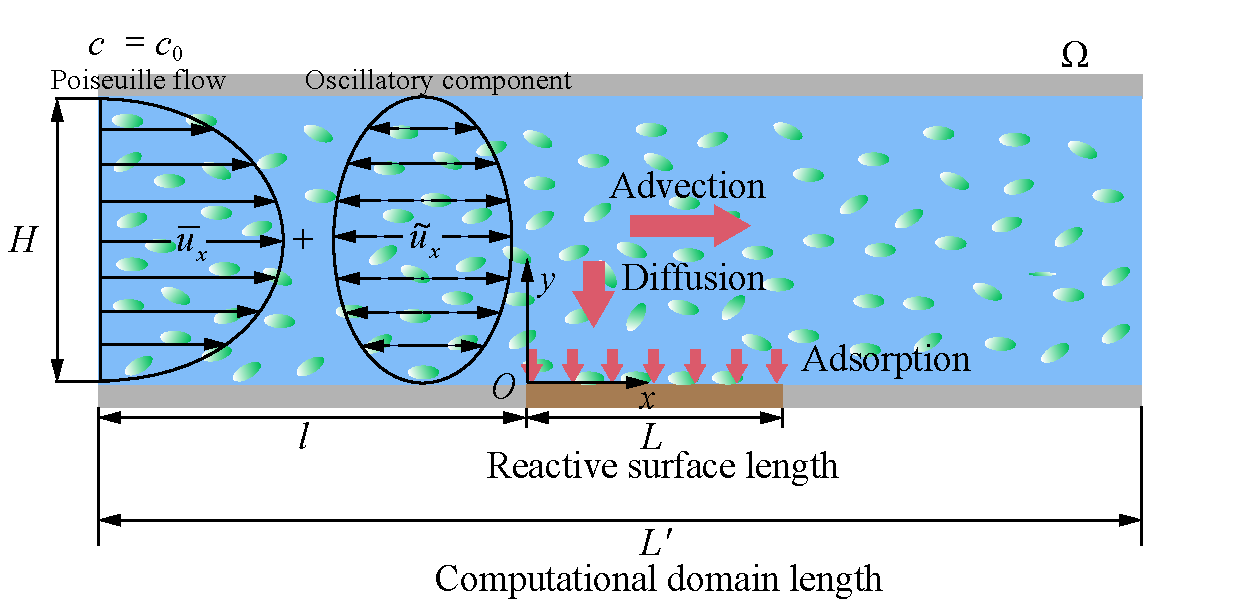
\includegraphics[width=0.65\textwidth]{figure/Schematic8.pdf}
\caption{Schematic and notation of the advection-diffusion-Langmuir adsorption processes in a two-dimensional oscillatory flow between two parallel planes. Adsorbates (molecules and particles) of concentration $c_0$ are introduced from the inlet of the 2-D channel, i.e., $x = -l$, into the flow. When adsorbates are advected along with the fluids into the reactive surface area starting at $O$, the concentration of free adsorbates adjacent to the surface decreases due to the adsorption at the surface. {\color{magenta}(use only $O$)} Then the bulk adsorbates spontaneously diffuse toward the surface in response to the concentration gradient across the flow. In general, the coupling of these three processes of advection, diffusion, and adsorption, modifies the concentration distribution of adsorbates in the flow. {\color{magenta}(what is $\Omega$? delete $r$ in the figure)}}
\label{fig:Schematic}
\end{center}
\end{figure}

{\color{blue}
We establish a two-dimensional model to systematically investigate the coupling between oscillatory flow advection-diffusion and boundary chemical reactions in mass transport processes, as illustrated in figure~\ref{fig:Schematic}. We consider a pressure-driven flow in a 2D channel (height $H$ $\times$ length $L'$) featuring a reactive surface of length $L$. The flow is governed by a composite pressure gradient $G = G_1 + G_2 \sin(\omega t)$, where $G_1$ represents the steady component and $G_2 \sin(\omega t)$ the oscillatory counterpart. Here, $\omega$ is the angular frequency of oscillation. The distance between the reactive surface and the channel inlet is defined as $l$. At the inlet ($x=-l$), we impose adsorbates with uniform concentration $c_0$ as the initial boundary condition.
%We introduce adsorbates at a uniform concentration $c_0$ at the inlet ($x=0$) of a two-dimensional channel (height $H$ $\times$ length $L'$) with a reactive surface of length $L$, in a flow driven by a pressure gradient $G$. Here, $G$ is composed of a steady component $G_1$ and an oscillatory component $G_2 \sin(\omega t)$. 
The velocity distribution of the carrier fluid in the oscillatory flows between two parallel planes can be analytically described as 
%改为subcase \begin{subnumcases} {\label{Boundary}}
% \begin{subequations}
% \begin{empheq}[left=\empheqlbrace]{align}
% u_x &= \begin{aligned}[t]
% &\frac{G_1}{2 \rho \nu}(yH - y^2)
% + \mathrm{Re} \left\{ \frac{G_2}{i \rho \omega}
% \left[ 1 - \frac{\cosh\left( \sqrt{\frac{\omega}{2\nu}}(1+i)(y-H/2) \right)}
%              {\cosh\left( \sqrt{\frac{\omega}{2\nu}}(1+i)H/2 \right)} \right]
% e^{i \omega t} \right\} \\
% &= \frac{G_1}{2 \rho \nu} (yH - y^2) + \frac{G_2}{\rho \omega} f(\alpha,y,t) \\
% &= \overline{u_x} + \widetilde{u_x},
% \end{aligned} \label{eq:ux_all} \\
% u_y& = 0, \label{eq:uy}
% \end{empheq}
% \end{subequations}
\begin{subequations}
\begin{empheq}[left=\empheqlbrace]{align}
u_x &= \frac{G_1}{2\rho v}(yH - y^2) + \text{Re}\left\{ \frac{G_2}{ip\omega} \left[ 1 - \frac{\cosh\left(\sqrt{\frac{\omega}{2v}}(1+i)(y-H/2)\right)}{\cosh\left(\sqrt{\frac{\omega}{2v}}(1+i)H/2\right)} \right] e^{i\omega t} \right\} \nonumber \\
    &= \frac{G_1}{2\rho v}(yH - y^2) + \frac{G_2}{\rho\omega}f(\alpha, y, t) \nonumber \\
    &= u_x + \bar{u}_x, \label{eq:ux_all} \\
u_y &= 0,  \label{eq:uy}
\end{empheq}
\end{subequations}
with 
\begin{align}
f(\alpha,y,t) &= \frac{1}{ \cos(2 \alpha) + \cosh(2 \alpha) } \bigg\{ \cos(2 \alpha) \sin(\omega t) + \cosh(2 \alpha) \sin(\omega t)  \notag\\
              &\quad + 2\cos\left(\frac{\alpha (y-H/2)}{H/2}\right) \cos(\omega t) \cosh\left(\frac{\alpha (y-H/2)}{H/2}\right) \sin(\alpha) \sinh(\alpha) \notag \\
              &\quad - 2 \sin(\alpha) \sin\left(\frac{\alpha (y-H/2)}{H/2}\right) \sin(\omega t) \sinh(\alpha) \sinh\left(\frac{\alpha (y-H/2)}{H/2}\right)  \notag \\
              &\quad - 2 \cos(\alpha) \cosh(\alpha)  \bigg[ \cos\left(\frac{\alpha (y-H/2)}{H/2}\right) \cosh\left(\frac{\alpha (y-H/2)}{H/2}\right) \sin(\omega t)  \notag \\
              &\quad  + \cos(\omega t) \sin\left(\frac{\alpha (y-H/2)}{H/2}\right) \sinh\left(\frac{\alpha (y-H/2)}{H/2}\right) \bigg] \bigg\},
\end{align}
where
%$G_1$ is the amplitude of the constant pressure gradient driving the steady flow [Pa/m],
%$G_2$ is the amplitude of the oscillating pressure gradient driving the unsteady flow [Pa/m],
$\rho$ is the fluid density,
%[kg/m³],
%$\omega$ is the angular frequency of oscillation [rad/s],
and $\nu$ is the kinematic viscosity of the fluid
%[m²/s] 
\citep{thomas2011linear,ma2017theoretical,westerhof2018snapshots}.
Here, the dimensionless parameter Womersley number $\alpha$ is defined as
\begin{equation}
\alpha = h\sqrt{\omega/2 \nu}.
\end{equation}
Physically, $\alpha$ represents the ratio of the transient inertial force to the viscous force \citep{womersley1955method}.  Note that the first term on the right-hand side of Eq.~\eqref{eq:ux_all} corresponds to the steady laminar flow component, or plane Poiseuille flow, driven by a constant pressure gradient through a 2-D channel \citep{Huang2023,Huang2024}. 
%We have investigated this kind of advection–diffusion–Langmuir adsorption processes numerically by the finite difference and physics-informed neural networks methods in detail in our previous study (\cite{Huang2023,Huang2024}).
%{\color{magenta}(add our previous paper for reference. Done)} 
The second term accounts for the contribution of the oscillatory flow component.
%{\color{red}
%Add a figure for velocity profiles of terms $y^*(1-y^*)$ and $\dfrac{1}{\alpha^2} f^*(\alpha^*, y^*, t^*)$. }

%Figure~\ref{fig:f_a_1} presents the spatial profiles of the steady term $\overline{u_x}$ and the oscillatory term $\widetilde{u_x}$ at four distinct phases, $t = \nicefrac{1}{8}T, \nicefrac{1}{4}T, \nicefrac{3}{8}T, \nicefrac{1}{2}T$, where the oscillation period is defined as $T = 2\pi/\omega$. The oscillatory velocity component $\widetilde{u_x}$ demonstrates significant dependence on both the dimensionless parameter $\alpha$ and temporal phase $t$. Under small $\alpha$ values, the velocity profile maintains its parabolic characteristics throughout the oscillation cycle (figure~\ref{fig:f_a_1}$b$). {\color{magenta}(relate the texts with figures b--d)} With moderate $\alpha$, a periodic alternation between curvature inversion and profile flattening emerges. At elevated $\alpha$ magnitudes, the flow develops quasi-flat velocity distributions accompanied by boundary-localized velocity extrema, due to the Richardson annular effect \citep{richardson1929transverse}. The numerical results presented agree with the velocity profiles reported by \cite{ma2017theoretical}.

Figure~\ref{fig:f_a_1} presents the spatial profiles of the steady term $\overline{u}_x$ and the oscillatory term $\widetilde{u}_x$ at four representative phases of the oscillation cycle, namely $t = \frac{1}{8}T$, $\frac{1}{4}T$, $\frac{3}{8}T$, and $\frac{1}{2}T$, where the period is defined as $T = 2\pi/\omega$. The velocities are normalized by the maximum centerline velocity $u_{\rm c}$, and their profiles are shown for different values of the Womersley number $\alpha$.
Figure~\ref{fig:f_a_1}($a$) illustrates the purely steady Poiseuille flow profile of $\overline{u}_x$, which remains parabolic and time-independent. In contrast, figure~\ref{fig:f_a_1}($b$) displays the oscillatory flow at $\alpha = 0.625$, where the velocity profile retains a nearly parabolic shape at all phases, but changes with time. When $\alpha = 3$ (figure~\ref{fig:f_a_1}($c$)), the profiles begin to shift more noticeably between different phases and show alternating bending directions and a gradual flattening of the center, indicating increased inertial influence. For large $\alpha = 6$ (figure~\ref{fig:f_a_1}($d$)), 
the flow develops a nearly flat profile in the middle of the channel, with strong peaks near the walls. This is a typical feature of high-frequency oscillatory flow known as the Richardson annular effect \citep{richardson1929transverse}. The numerical results shown are in good agreement with those reported by \cite{ma2017theoretical}.

%{\color{green}
%To illustrate the characteristics of the two velocity components, figure~\ref{fig:f_a_1} presents the spatial profiles of the steady term $\overline{u_x}$ and the oscillatory term $\widetilde{u_x}$ at four representative time points, $t = \nicefrac{1}{8}T, \nicefrac{1}{4}T, \nicefrac{3}{8}T, \nicefrac{1}{2}T$, where the oscillation period is defined as $T = 2\pi/\omega$. The magnitude and shape of the oscillatory component $\widetilde{u_x}$ depend strongly on the dimensionless parameter $\alpha$ and time $t$, exhibiting transitions from parabolic to flattened or even multi-extremum profiles. At small $\alpha$, the flow remains parabolic throughout the cycle; at moderate $\alpha$, curvature and flatness alternate; and at large $\alpha$, the profiles become nearly flat with wall-localized extrema due to the Richardson annular effect (\cite{richardson1929transverse}). The numerical results shown here reproduce the velocity profiles reported by \cite{ma2017theoretical} with exact agreement.
%}

\begin{figure}
\begin{center}
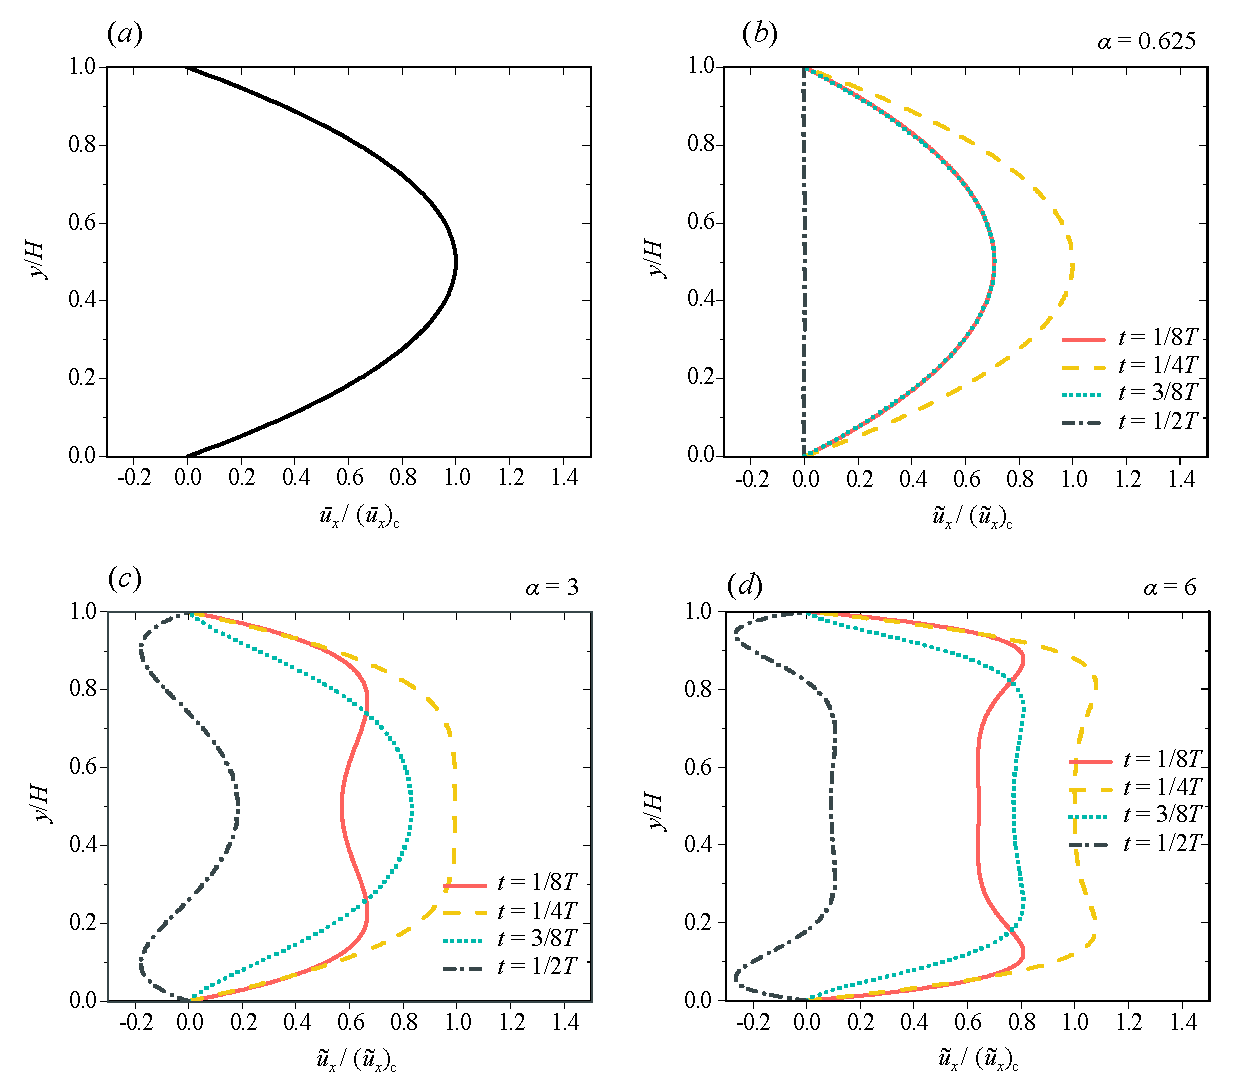
\includegraphics[width=0.9\textwidth]{figure/f_a_v5.pdf}
\caption{{\color{blue}Normalized velocity profiles of ($a$) the steady laminar component $\overline{u}_x$, and the oscillatory term $\widetilde{u}_x$ at ($b$) $\alpha = 0.625$, ($c$) $\alpha = 3$, and ($d$) $\alpha = 6$ during the first half of their oscillation cycles. The corresponding maximum velocity at the central line is denoted by the subscript $c$. }
%{\color{magenta}(note the differences of $\overline{u_x}$ and $\widetilde{u_x}$ in the figure and the text.)}}
%Comparison of velocity profiles: the steady laminar component $\overline{u_x}$ and the oscillatory term $\widetilde{u_x}$ at different instants during the first half of the oscillation cycle for various $\alpha$. The maximum velocity at the central line is defined as $u_{\rm c}$. (a) Steady flow velocity profile; (b) Oscillatory flow with $\alpha = 0.625$; (c) Oscillatory flow with $\alpha = 3$; (d) Oscillatory flow with $\alpha = 6$.
}

\label{fig:f_a_1}
\end{center}
\end{figure}


Then the 2-D advection-diffusion equation of the concentration $c$ in a Cartesian reference frame becomes 
\begin{equation} {\label{Govern}}
{\frac{{\partial}c}{{\partial}t}} = {D \left( \frac{{\partial}^2 c}{{\partial}{x}^2} + \frac{{\partial}^2 c}{{\partial}{y}^2} \right) 
  - u_{x}\frac{{\partial}c}{{\partial}x}},
\end{equation}
where $D$ is the diffusion coefficient of the adsorbates \citep{Huang2023,Huang2024}. Assuming that the reaction process satisfies the Langmuir adsorption model, in cases where a continuous monolayer of adsorbed molecules or particles covers a homogeneous flat solid surface, a complete set of boundary conditions is given as 
\begin{subnumcases} {\label{Boundary}}
 D\frac{{\partial}c}{{\partial}y} = \frac{{\partial}b}{{\partial}t} =  k_{\rm a}~c_{\rm s}~(b_{\max}-b) - k_{\rm d} b, & for $y=0$ and $0 \leq x \leq L$,\label{BC(a)}\\
c = c_0, & for $x = -l$,\label{BC(b)} \\
{\bf{n}}\cdot\nabla c = 0, b = 0, & for all other boundary surfaces, {\label{BC(c)} }
\end{subnumcases}
where $c_{\rm s} = c\mid_{y = 0}$ is the concentration of free adsorbates in the bulk solution adjacent to the surface, $k_{\rm a}$ and $k_{\rm d}$ are the adsorption and desorption rate constants, respectively, and $b$ is the surface concentration of the bound adsorbates, with a maximum $b_{\max}$ \citep{Huang2023,Huang2024}. Note that the dimension of the adsorption rate constant $k_{\rm a}$ is $[{\rm N^{-1} \cdot L^{3} \cdot T^{-1}}]$, and the dimension of the desorption rate constant $k_{\rm d}$ is $[{\rm T}^{-1}]$\footnote{Here, [N] denotes the amount of substance, [L] denotes the dimension of length, and [T] denotes the dimension of time.}.
%, representing the amount of adsorbates desorbed on the saturation surface per unit time. 
Equation (\ref{BC(c)}) accounts for the zero Neumann boundary condition, where {\bf{n}} is the unit normal vector.

%We set up a 2-D model to systematically study the coupling of the mass transport processes between the advection-diffusion in the oscillatory flows and the chemical reaction on the boundary, as shown in figure~\ref{fig:Schematic}.
%We inject adsorbates with uniform concentration $c_0$ into a flow with a volume flow rate per unit width $Q$, through a 2-D
%channel (height $H$ $\times$ length $L'$) with a reactive surface of length $L$. The distance between the reactive surface and the channel inlet is set to $l=O_1O_2$.
% When $W \gg H$,  the flow velocities in the span direction are negligible, and the system becomes essentially two-dimensional. 
%This steady (laminar) flow driven by a constant pressure gradient through a 2-D channel is called the plane Poiseuille flow, whose velocity distribution has an analytical solution, i.e. ${u_x} = {({6Q}/{H^3})y(H-y)}$ and ${u_y} = {0}$, where $u_x$ and $u_y$ are the velocity components of the carrier fluid along the $x$ and $y$ directions, respectively. 

%Then the 2-D advection-diffusion equation of the concentration $c$ in a Cartesian reference frame ${{{\partial}c}/{{\partial}t}} = {D({{\partial}^2 c}/{{\partial}{x}^2} + {{\partial}^2 c}/{{\partial}{y}^2}) - (u_x{{\partial}c}/{{\partial}x} + u_y{{\partial}c}/{{\partial}y})}$, where $D$ is the diffusion coefficient of the adsorbates, becomes
%\begin{equation} {\label{Govern}}
%{\frac{{\partial}c}{{\partial}t}} = {D \left( \frac{{\partial}^2 c}{{\partial}{x}^2} + \frac{{\partial}^2 c}{{\partial}{y}^2} \right) 
%  - u_{x}\frac{{\partial}c}{{\partial}x}},
%\end{equation}
%where
%\begin{align}    
%\label{eq:u_x}
%u_x(y,t) &= \frac{G_1}{2 \rho \nu}(yH-y^2)+ {\rm Re} \left\{\frac{G_2}{i\rho \omega}\left[{1-\frac{{\rm cosh}\left(\sqrt{\omega/2\nu}(1+i)(y-H/2)\right)} {{\rm cosh}\left(\sqrt{\omega/2\nu}(1+i)H/2\right)}}\right] e^{i \omega t}\right\} \notag \\
%         &= \frac{G_1}{2 \rho \nu} \left( yH-y^2 \right) + \frac{G_2}{\rho \omega} f(\alpha,y,t),
%\end{align}
%with 
%\begin{align}
%f(\alpha,y,t) &= \frac{1}{ \cos(2 \alpha) + \cosh(2 \alpha) } \bigg\{ \cos(2 \alpha) \sin(\omega t) + \cosh(2 \alpha) \sin(\omega t)  \notag\\
%              &\quad + 2\cos\left(\frac{\alpha (y-H/2)}{H/2}\right) \cos(\omega t) \cosh\left(\frac{\alpha (y-H/2)}{H/2}\right) \sin(\alpha) \sinh(\alpha) \notag \\
%              &\quad - 2 \sin(\alpha) \sin\left(\frac{\alpha (y-H/2)}{H/2}\right) \sin(\omega t) \sinh(\alpha) \sinh\left(\frac{\alpha (y-H/2)}{H/2}\right)  \notag \\
%              &\quad - 2 \cos(\alpha) \cosh(\alpha)  \bigg[ \cos\left(\frac{\alpha (y-H/2)}{H/2}\right) \cosh\left(\frac{\alpha (y-H/2)}{H/2}\right) \sin(\omega t)  \notag \\
%              &\quad  + \cos(\omega t) \sin\left(\frac{\alpha (y-H/2)}{H/2}\right) \sinh\left(\frac{\alpha (y-H/2)}{H/2}\right) \bigg] \bigg\}.
%\end{align}
%Here, the dimensionless parameter Womersley number ($\alpha$) is
%defined as
%\begin{equation}
%\alpha = h\sqrt{\omega/2 \nu}.
%\end{equation}
%Physically, $\alpha$ represents the ratio of the transient inertial force to the viscous force. 




%Assuming that the reaction process satisfies the Langmuir adsorption model, in cases where a continuous monolayer of adsorbed molecules or particles covers a homogeneous flat solid surface, a complete set of boundary conditions are given as
%\begin{subnumcases} {\label{Boundary}}
% D\frac{{\partial}c}{{\partial}y} = \frac{{\partial}b}{{\partial}t} =  k_{\rm a}~c_{\rm s}~(b_{\max}-b) - k_{\rm d} b, & for $y=0$ and $0 \leq x \leq L$,\label{BC(a)}\\
%c =c_0, & for $x=-l$,\label{BC(b)} \\
%{\bf{n}}\cdot\nabla c = 0, b = 0, & for all other boundary surfaces, {\label{BC(c)} }
%\end{subnumcases}
%where $c_{\rm s} = c\mid_{y = 0}$ is the concentration of free adsorbates in the bulk solution adjacent to the surface, $k_{\rm a}$ and $k_{\rm d}$ are the adsorption and desorption rate constants, respectively, and $b$ is the surface concentration of the bound adsorbates, with a maximum $b_{\max}$. Here the dimension of adsorption rate constant $k_{\rm a}$ is $[{\rm N^{-1} \cdot M^{3} \cdot T^{-1}}]$, representing the amount of adsorbates adsorbed on the blank surface per unit concentration per unit time; and the dimension of desorption rate constant $k_{\rm d}$ is $[{\rm T}^{-1}]$, representing the amount of adsorbates desorbed on the saturation surface per unit time. Equation (\ref{BC(c)}) accounts for the zero Neumann boundary condition, and {\bf{n}} is the unit normal vector.

%\section{Nondimensionlization and numerical method}
%\label{sec:3}

To systematically investigate the effects of control parameters on the process dynamics, we solve the advection-diffusion equation in its dimensionless form
\begin{align}
\frac{{\partial}c^*}{{\partial}t^*} &= \lambda^2 \frac{{\partial}^2 c^*}{{\partial}{x^*}^2} + 
       \frac{{\partial}^2 c^*}{{\partial}{y^*}^2} 
     - \lambda Pe_1~y^*\left(1-y^*\right)\frac{{\partial}c^*}{{\partial}x^*} - \lambda Pe_2 \frac{1}{\alpha^2}f^*(\alpha,y^*,t^*) \frac{{\partial}c^*}{{\partial}x^*}, \label{Non_Govern}  
\end{align}
with
\begin{align}
f^*(\alpha,y^*,t^*) &= \frac{1}{ \cos(2 \alpha) + \cosh(2 \alpha) } \bigg\{ \cos(2 \alpha) \sin(2 \alpha^2\,Sc ~t^*  ) + \cosh(2 \alpha) \sin(2 \alpha^2\, Sc ~t^*  )  \notag \\
              &\quad + 2\cos\left(\frac{\alpha (y^*-0.5)}{0.5}\right) \cos(2 \alpha^2 Sc  ~t^*  ) \cosh\left(\frac{\alpha (y^*-0.5)}{0.5}\right) \sin(\alpha) \sinh(\alpha) \notag \\
              &\quad - 2 \sin(\alpha) \sin\left(\frac{\alpha (y^*-0.5)}{0.5}\right) \sin(2 \alpha^2\, Sc  ~t^*  ) \sinh(\alpha) \sinh\left(\frac{\alpha (y^*-0.5)}{0.5}\right) \notag \\
              &\quad - 2 \cos(\alpha) \cosh(\alpha)  \bigg[ \cos\left(\frac{\alpha (y^*-0.5)}{0.5}\right) \cosh\left(\frac{\alpha (y^*-0.5)}{0.5}\right) \sin(2 \alpha^2 \,Sc~t^* ) \notag \\
              &\quad + \cos(2 \alpha^2\, Sc  ~t^* ) \sin\left(\frac{\alpha (y^*-0.5)}{0.5}\right) \sinh\left(\frac{\alpha (y^*-0.5)}{0.5}\right) \bigg] \bigg\},
\end{align}
where $\lambda=H/L$, $Sc = \nu/D$, using the normalized variables ${c^*} = c/c_0$, $x^* = x/L$, ${y^*} = y/H$, and ${t^*} = t/(H^2/D)$, where $H^2/D$ represents the characteristic diffusion time scale. The nondimensional parameters $Pe_1$ and $Pe_2$ are the P\'{e}clet numbers corresponding to the steady and oscillatory flow components, respectively
\begin{subequations}
\begin{empheq}[left=\empheqlbrace]{align}
Pe_1 &= \frac{G_1 H^3}{2 \mu D}, \label{eq:Pe1} \\
Pe_2 &= \frac{G_2 H^3}{2 \mu D}, \label{eq:Pe2}
\end{empheq}
\end{subequations}
where $\mu$ is the dynamic viscosity of the carrier fluid. They determine the ratio of convective flux to diffusive flux, or equivalently, represent the ratio of the diffusion time scale to the advection time scale.

%To systematically study the influence of the control parameters on the dynamics characteristics of the process, using nondimensional parameters ${c^*} = c/c_0$, $x^* = x/L$, ${y^*} = y/H$, and ${t^*} = t/(H^2/D)$, where $H^2/D$ represents the characteristic diffusion time scale, we solve the governing equations in their nondimensional forms. 
%\begin{align}
%\frac{{\partial}c^*}{{\partial}t^*} &= \lambda^2 \frac{{\partial}^2 c^*}{{\partial}{x^*}^2} + 
%       \frac{{\partial}^2 c^*}{{\partial}{y^*}^2} 
%     - \lambda Pe_1~y^*(1-y^*)\frac{{\partial}c^*}{{\partial}x^*} - \lambda Pe_2 \frac{1}{\alpha^2}f^*(\alpha,y^*,t^*) \frac{{\partial}c^*}{{\partial}x^*}, \label{Non_Govern}  
%\end{align}
%with
%\begin{align}
%f^*(\alpha,y^*,t^*) &= \frac{1}{ \cos(2 \alpha) + \cosh(2 \alpha) } \bigg\{ \cos(2 \alpha) \sin(2 \alpha^2\,Sc ~t^*  ) + \cosh(2 \alpha) \sin(2 \alpha^2\, Sc ~t^*  )  \notag \\
%              &\quad + 2\cos\left(\frac{\alpha (y^*-0.5)}{0.5}\right) \cos(2 \alpha^2 Sc  ~t^*  ) \cosh\left(\frac{\alpha (y^*-0.5)}{0.5}\right) \sin(\alpha) \sinh(\alpha) \notag \\
%              &\quad - 2 \sin(\alpha) \sin\left(\frac{\alpha (y^*-0.5)}{0.5}\right) \sin(2 \alpha^2\, Sc  ~t^*  ) \sinh(\alpha) \sinh\left(\frac{\alpha (y^*-0.5)}{0.5}\right) \notag \\
%              &\quad - 2 \cos(\alpha) \cosh(\alpha)  \bigg[ \cos\left(\frac{\alpha (y^*-0.5)}{0.5}\right) \cosh\left(\frac{\alpha (y^*-0.5)}{0.5}\right) \sin(2 \alpha^2 \,Sc~t^* ) \notag \\
%              &\quad + \cos(2 \alpha^2\, Sc  ~t^* ) \sin\left(\frac{\alpha (y^*-0.5)}{0.5}\right) \sinh\left(\frac{\alpha (y^*-0.5)}{0.5}\right) \bigg] \bigg\},
%\end{align}
%where $\lambda=H/L$, $Sc = \nu/D$. 

%The nondimensional parameters $Pe_1$ and $Pe_2$ are the P\'{e}clet numbers corresponding to the steady and oscillatory flows, respectively. They determine the ratio of convective flux to diffusive flux, or equivalently represent the ratio of the diffusion time scale to the advection time scale. For a pressure-driven flow,

%\begin{subequations}
%\begin{empheq}[left=\empheqlbrace]{align}
%Pe_1 &= \frac{G_1 H^3}{2 \mu D}, \label{eq:Pe1} \\
%Pe_2 &= \frac{G_2 H^3}{2 \mu D}. \label{eq:Pe2}
%\end{empheq}
%\end{subequations}

%where $G_1$ is the constant pressure gradient [Pa/m], $G_2$ is the amplitude of the oscillating pressure gradient [Pa/m], $H$ is the channel height [m], $\mu$ is the dynamic viscosity [Pa·s], and $D$ is the molecular diffusion coefficient [m$^2$/s].


Accordingly, the boundary conditions are nondimensionalized as
% \begin{subnumcases} {\label{NBC} }
%  {F = \epsilon}\frac{{\partial}c^*}{{\partial}y^*}=\frac{{\partial}\eta}{{\partial}t^*}=\epsilon ~ Da ~ [c_{\rm s}^*(1-\eta)-\frac{1}{K_0}\eta], & for $y^*=0$ and $0 \leq x^* \leq 1$,\label{NBC(a)}\\
%  c^* =1, & for $-l^*\leq x^* \leq 0$, $t^* =0$, \label{NBC(b)}\\
%  {\bf n}\cdot\nabla c^* = 0, \eta = 0, & for all other boundary surfaces, \label{NBC(c)}
% \end{subnumcases}
\begin{subnumcases} {\label{DBC} }
 {F = \epsilon}\frac{{\partial}c^*}{{\partial}y^*}=\frac{{\partial}\eta}{{\partial}t^*}=\epsilon \, Da \,\left[c_{\rm s}^*(1-\eta)-\frac{1}{K_0}\eta\right], & for $y^*=0$ and $0 \leq x^* \leq 1$, \label{DBC_a} \\
  c^* =1, & for $x^* = -l^*$,\label{DBC_b}\\
 {\bf n}\cdot\nabla c^* = 0, \,\eta = 0, & for all boundary surfaces. \label{DBC_c}
\end{subnumcases}
The initial conditions are nondimensionalized as
\begin{subnumcases} {\label{IBC} }
 c^* =1, & for $x^* = -l^*$,\label{IBC_a} \\
 c^* = 0, \,\eta = 0, & for all other zones, \label{IBC_b}
\end{subnumcases}
%where $\eta = b/{b_{\max}}$ is the surface concentration normalized by the maximum surface concentration, $c_{\rm s}^* = c_{\rm s}/c_{0}$ is the nondimensional concentration of free adsorbates in the bulk solution adjacent to the channel surface, $ Da = k_{\rm a} b_{\max} H/D$ is the Damk\"{o}hler number which gives the ratio between reaction and diffusion flux, $\epsilon = c_{0}H/b_{\max}$ is the relative adsorption capacity, corresponding to the relative density of adsorbates between the bulk and the fully saturated surfaces (a measure of surface adsorption capacity relative to the bulk concentration), $K_0 = k_{\rm a} c_{0}/k_{\rm d}$ is the chemical equilibrium constant, $l^*=l/L'$, $\lambda' = H/L'$. 
%the average surface concentration on the reactive surface $b_{\rm ave} = {\int_{0}^{L} b(x) {\rm d}x}/L$ and the adsorption flux ${\partial b_{\rm ave}}/{\partial t}$ can be normalized as $\eta_{\rm ave}={\int_{0}^{1} \eta(x^*) {\rm d}x^*}$ and $F_{\rm ave} = {\int_{0}^{1} F(x^*) {\rm d}x^*} = {\partial \eta_{\rm ave}}/{\partial t^*}$, respectively. {\color{red}(language narratives need  change!)} 
where the surface concentration $b$ is nondimensionalized as $\eta = b / b_{\max}$, in which $b_{\max}$ denotes the maximum surface concentration; the concentration of free adsorbates in the bulk fluid adjacent to the surface is expressed in nondimensional form as $c_{\rm s}^* = c_{\rm s}/c_0$, with $c_0$ representing the inlet bulk concentration.
The Damköhler number is defined as $Da = k_{\rm a} b_{\max} H / D$, quantifying the ratio of the characteristic adsorption rate to the diffusive transport rate. The parameter $\epsilon = c_0 H / b_{\max}$ characterizes the relative adsorption capacity, representing the ratio of bulk-phase adsorbate density to that of a fully saturated surface. The dimensionless equilibrium constant is given by $K_0 = k_{\rm a} c_0 / k_{\rm d}$. Additionally, we define $l^* = l / L'$ and $\lambda' = H / L'$.

We numerically solve the advection-diffusion equation (Eq.~\eqref{Non_Govern}) subject to the boundary condition specified in Eq.~\eqref{DBC_a}, employing a finite difference method that extends our established computational framework presented in \cite{Huang2023}. Note that the analytical solution $ f^*(\alpha, y^*, t) $ in Eq.~\eqref{Non_Govern}, which governs the oscillatory dynamics, exhibits explicit temporal dependence. We briefly describe the algorithms as follows.

The computational domain is defined as $\Omega = (0, L') \times (0, H)$ and employs a uniform grid spacing $h = L'/N_x = H/N_y$, where $N_x$ and $N_y$ represent the number of computational cells in the $x$ and $y$ directions, respectively. The nodal positions are determined by 
\begin{equation}
 (x_i^*, y_j^*) = (ih, jh) \quad \text{for} \quad 
\begin{cases} 
i = 0,1,...,N_x, \\
j = 0,1,...,N_y. 
\end{cases}   
\end{equation}
The dimensionless variables are discretized as free adsorbate concentration $c^*_{i,j}=c^*(x^*_i,y^*_j)$, bound adsorbate surface concentration $\eta_{i}=\eta(x^*_i)$, and oscillatory flow component $ f_j^* = f^*(\alpha, y_j^*, t)$. 

%We then solve Eq.~\eqref{Non_Govern} with boundary condition of Eq.~\eqref{DBC_a} using a finite difference method. The numerical approach is similar to the work we did in \cite{Huang2023}. Note that the analytical solution $f^*(\alpha, y^*, t)$ in Eq. \eqref{Non_Govern} that governs the oscillating behaviors is a function of time $t$. We briefly describe the algorithms as follows.
% Furthermore, we did the independence tests, as shown in Fig. XX.  
% There are several numerical methods that can be used to solve the ADR equations,\cite{?} here we solve the nondimensional advection-diffusion Eq.(\ref{Non_Govern}), coupled with the boundary conditions Eqs.(\ref{NBC}) by a finite difference method. 

%Let the computational domain be $\Omega=(0,L')\times(0,H)$ and, for convenience, we define the uniform mesh size $h=L'/N_x=H/N_y$, where integers $N_x$ and $N_y$ are the numbers of cells in $x-$ and $y-$directions, respectively. 
%By this setting, we have a rectangle computational domain as $L = m H$, where $m$ is an integer.
%The location of the node ($i,j$) is then $(x^*_i=ih, y^*_j=jh)$, where $i=0,..., N_x$, and $j=0,..., N_y$. With the above definitions, the nondimensional concentration of free adsorbates $c$, the surface concentration of bound adsorbates $\eta$ and the analytical solution of oscillatory flow component $f^*(\alpha, y^*, t)$ are discretely denoted by $c^*_{i,j}=c^*(x^*_i,y^*_j)$,  $\eta_{i}=\eta(x^*_i)$ and $ f_j^* = f^*(\alpha, y_j^*, t)$, respectively.   

Let $c_{i,j}^{*n}$ and $\eta_{i}^n$ denote the discrete approximations of $c^*(x^*_i, y^*_j)$ and $\eta(x^*_i)$ at dimensionless time $t^*_n=n\Delta t^*$, where $\Delta t^*$ represents the time step and $n$ counts iterations between \textit{Step 1} to \textit{Step 3} described below. The complete time-marching algorithm for $c^*$ and $\eta$ updates comprises three core operations per time step:



%Let $c_{i,j}^n$ and $\eta_{i}^n$ be approximations of $c^*(x^*_i, y^*_j)$ and $\eta(x^*_i)$ at time $t^*_n$, where $t^*_n=n\Delta t^*$, with $\Delta t^*$ being the time step and $n$ the number of iterations from \textit{Step 1.} to \textit{Step 3.} 
%To ensure numerical stability, the time step $\Delta t^*$ must satisfy the condition $\Delta t^*/h \leq 0.25$, following the Courant–Friedrichs–Lewy (CFL) criterion in \cite{courant1967partial}.
%A smaller time step leads to more iterations and thus increased computational cost.
%In this study, the time step is empirically set to $\Delta t^*/h = 0.2$ for $Pe < 10^3$ and $\Delta t^*/h = 5/Pe$ for $Pe \geq 10^3$, to balance computational efficiency and numerical stability. (Here, how to select $\delta t^*$ may change, to satisfy the CFL condition, i.e. $|a|\Delta t^*/h\le 1$ ). The full algorithms to calculate $c^*$ and $\eta$ in a one-time step are as follows:

\noindent \textit{Step 1.} Calculate $\eta_i^{n+1}$ with Eq.~(\ref{DBC_a}) by a forward Euler method,
\begin{equation}{\label{Forward Difference}}
\eta_i^{n+1} = \eta_i^n + \Delta t^* \,\epsilon \, Da \left[ {c^*_{\rm s}}_i(1-\eta_i^n) - 1/K_0 \,\eta_i^n \right],  \quad \text{for } \ i = 0,...,N_x.
\end{equation}

\noindent \textit{Step 2.} Apply the boundary conditions Eqs.~(\ref{DBC_b}) and (\ref{DBC_c}) for $c_{i,j}^{*\,n}$.

\noindent \textit{Step 3.} Update $c_{i,j}^{*\,n}$ by discretizing Eq.~(\ref{Non_Govern}) with

\begin{align} \label{C_Difference}
\left\{\begin{aligned}
 P_{i,j} &= {\frac{c_{i+1,j}^{*\,n} + c_{i-1,j}^{*\,n} - 2c_{i,j}^{*\,n}}{h^2}} + {\frac{c_{i,j+1}^{*\,n} + c_{i,j-1}^{*\,n} - 2c_{i,j}^{*\,n}}{h^2}},\\
 Q_{i,j} &= a^{+} \frac{c_{i,j}^{*\,n} - c_{i-1,j}^{*\,n}}{h} + a^{-} \frac{c_{i+1,j}^{*\,n} - c_{i,j}^{*\,n}}{h}, \\
 c_{i,j}^{*\,n+1} &= c_{i,j}^{*\,n} + \Delta t^* \left( P_{i,j}-Q_{i,j} \right), \\  
\end{aligned}\right.
\end{align}
where $a^{+} = \max \left(a, \, 0 \right)$ and $a^{-} = \min \left(a, \, 0 \right)$, in which $a     = Pe_1~y^*_j (1-y^*_j)+ Pe_2~f_j^{*\,n} / \alpha^2$.


%\begin{equation}
%    a^{+} = \max \left(a, \, 0 \right), \quad a^{-} = \min \left(a, \, 0 \right),
%\end{equation}
%in which
%\begin{equation}
%  a     = Pe_1~y^*_j (1-y^*_j)+ Pe_2~f_j^{*\,n} / \alpha^2.  
%\end{equation}
%\begin{align}
%   a^{+} &= \max \left(a, \, 0 \right), \quad a^{-} = \min \left(a, \, 0 \right), \notag \\
%   a     &= Pe_1~y^*_j (1-y^*_j)+ Pe_2~f_j^n / \alpha^2. \notag
%\end{align}

The time-marching algorithm completes one full temporal iteration through \textit{Steps 1--3}, updating both $c_{i,j}^{*n+1}$ and $\eta_i^{n+1}$. To ensure numerical stability, we adhere to the classical Courant-Friedrichs-Lewy (CFL) condition \citep{courant1967partial}, maintaining the dimensionless Courant number below a conservative empirical limit of $0.25$. While the original CFL condition provides the theoretical necessity for stability, this specific threshold is chosen to ensure robust convergence for the coupled bulk-surface reaction dynamics.

Furthermore, for cases involving oscillatory flow, the time step must be sufficiently small to resolve the rapid temporal variations of the flow field. We impose an additional constraint that each oscillation period, $T^* = 2\pi / (\alpha^2 Sc)$, must be resolved by at least 20 time steps. Consequently, we require $\Delta t \le 0.05 T^*$, which leads to the following restriction:
\begin{equation}
\Delta t \le \frac{\pi}{10 \alpha^2 Sc}.
\label{eq:dt_oscillation}
\end{equation}
In our simulations, we employ an adaptive time-stepping rule that dynamically adjusts $\Delta t$ to satisfy both the CFL stability criterion and the temporal resolution requirement of the oscillatory forcing, thereby achieving an optimal balance between accuracy and computational efficiency.

 
While maintaining explicit time integration for computational efficiency, the scheme ensures stability through upwind discretization of $Q_{i,j}$ in \textit{Step 3}, which is appropriate for the laminar flow regime considered here. The initial concentration distribution follows
%The initial concentration field $c^*$ is prescribed as
\begin{equation}
   c^*(x^*_i,y^*_j)\big|_{t=0}= \frac{1}{2}\left[-\frac{\tanh{(x^*_i - 3h)}}{\sqrt{2}\beta} + 1 \right],
\end{equation}
where $\beta = \frac{h}{\sqrt{2} \arctanh(0.9)}$. This profile establishes a well-defined buffer layer of characteristic thickness $6h$ adjacent to the inlet, facilitating a continuous transition of $c^*$ from unity at the upstream boundary to zero downstream, thereby mitigating numerical instabilities during initial transients.

To evaluate the progression of surface adsorption, we define the spatially averaged nondimensional surface concentration over the reactive surface $\eta_{\rm ave}$ as
\begin{equation}
\eta_{\rm ave} = \int_0^1 \eta(x^*)\,\mathrm{d}x^*,
\end{equation}
which, in the discrete form, is computed as
\begin{equation}
\eta_{\rm ave} = \frac{1}{N_x'} \sum \eta_i^n = \frac{1}{N_x \lambda'/\lambda} \sum \eta_i^n,
\end{equation}
where $N_x'$ denotes the number of spatial nodes within the reactive regime, and $\lambda'/\lambda$ accounts for the nondimensionalized length fraction.

To assess the accuracy of the numerical solution, we adopt a convergence criterion based on the relative difference between the instantaneous average surface concentration and its theoretical equilibrium value:
\begin{equation}
\frac{\eta_{\rm eq} - \eta_{\rm ave}}{\eta_{\rm eq}} < 10^{-3},
\end{equation}
where $\eta_{\rm eq} = K_0 / (K_0 + 1)$ is the nondimensional equilibrium coverage derived from Langmuir kinetics.

To characterize the adsorption dynamics, we define the saturation time $t_{0.99}^*$ as the first instance at which the average surface concentration reaches 99\% of its theoretical maximum value $\eta_{\rm eq}$. {\color{magenta}(add references. add discussion on .99 and .95 in appendix)} This definition is formalized as:
\begin{equation}
t_{0.99}^* = \min \{ t^* \mid \eta_{\rm ave}(t^*) \geq 0.99\, \eta_{\rm eq} \}.
\label{eq:saturation_time}
\end{equation}

In systems dominated by steady advection, $\eta_{\rm ave}(t^*)$ typically increases monotonically, making $t_{0.99}^*$ a unique and straightforward measure of the approach to equilibrium. {\color{magenta}(set two examples: see case ... in Sec. ...)} However, in oscillation-dominated regimes, the surface concentration may exhibit periodic fluctuations due to the unsteady shear and concentration boundary layers. In such cases, defining $t_{0.99}^*$ as the \textit{first} time the threshold is crossed ensures a robust and consistent metric that captures the characteristic timescale of the initial binding process. This choice allows for a meaningful comparison across a wide range of Womersley numbers ($\alpha$) and oscillatory P\'{e}clet numbers ($Pe_2$), where the onset of the saturation plateau is of primary interest for sensor response and diagnostic applications.

Based on this, the average adsorption flux $F_{\rm ave}$ is introduced to quantify the overall adsorption rate:
\begin{equation}
F_{\rm ave} = \frac{\eta_{\max}}{t_{0.99}^*},
\label{eq:Fave}
\end{equation}
which measures the time-averaged rate at which the surface becomes saturated under a specific condition.
}




%{\color{red}

%\textit{Steps 1--3} complete the calculation of $c_{i,j}^{n+1}$ and $\eta_i^{n+1}$ in one time step. 
%Although the scheme is explicit and algorithmically simple, numerical stability under small time steps is ensured by employing an upwind discretization for $Q_{i,j}$ in \textit{Step 3}, which is appropriate for the laminar flow regime considered here. 
%The initial concentration field $c^*$ is prescribed as
%\[
%c^*(x^*_i,y^*_j)\big|_{t=0}= \frac{1}{2}\left[-\frac{\tanh{(x^*_i - 3h)}}{\sqrt{2}\beta} + 1 \right],
%\quad \text{where} \quad \beta = \frac{h}{\sqrt{2} \arctanh(0.9)}.
%\]
%This smooth transition introduces a finite buffer layer of thickness $6h$ near the inlet, allowing $c^*$ to vary continuously from 1 to 0 and ensuring numerical stability at early times.

%A steady-state criterion is imposed based on the relative error between the spatially averaged surface concentration and its equilibrium value:
%\[
%\frac{\eta_{\rm eq} - \eta_{\rm ave}}{\eta_{\rm eq}} < 10^{-3},
%\]
%where $\eta_{\rm eq} = K_0 / (K_0 + 1)$ denotes the nondimensional surface concentration at equilibrium, and the spatial average is calculated as
%\[
%\eta_{\rm ave} = \frac{1}{N_x'} \sum \eta_i^n = \frac{1}{N_x \lambda'/\lambda} \sum \eta_i^n.
%\]

%}

% {\color{magenta}(describe the numerical scheme in the main text)}

\section{\label{sec:results}Overview of the advection-diffusion-Langmuir adsorption processes}


{\color{blue}

Using the numerical framework described in previous sections, we conduct a systematic parametric study across key dimensionless parameters, as shown in Table~\ref{tab:group}. The investigation focuses on four distinct steady P\'{e}clet numbers $Pe_1 = \{0, 10, 100, 1000\}$, with each group comprising a comprehensive $81 \times 81$ parameter sweep over two additional variables: $f \in [10^{-1},\;10^{6}] $ and $a \in [0.01,\ 10]$, enabling detailed analysis of their coupled effects. {\color{magenta}(parametric space changed)} This design results in 6,561 simulations per $Pe_1$ value, yielding a total of 26,244 distinct simulation cases. {\color{magenta}(number of cases changed)} These broad parametric ranges are carefully selected to encompass the diverse physical regimes observed in practical applications, as summarized in Table~\ref{tab:adr_applications}. The combination of high-resolution parameter sampling and multiple $Pe_1$ configurations provides robust coverage of both fundamental transport mechanisms and application-oriented scenarios.
{\color{magenta}(the choice of $l$. $l$ or $l^*$?)}{\color{brown}The length $l^*$, defined as the distance between the inlet boundary and the upstream edge of the reactive surface, is selected by balancing computational cost and boundary-condition effects. If $l^*$ is taken too large, the computational domain is unnecessarily enlarged without improving the solution near the reactive surface. If $l^*$ is too small, however, the Dirichlet condition imposed at the inlet may directly influence the flow and concentration fields in the vicinity of the reactive surface, especially under strong oscillatory flow, where the upstream disturbance penetrates farther into the domain. In the present study, $l^* = 0.125$ is adopted as a compromise.}


}

%With the help of the numerical technique mentioned above, we perform systematic simulations to explore the governing parameter space. A total of 6,724 simulation cases were conducted. These cases are organized into four main groups, each corresponding to a distinct value for the steady P\'{e}clet number, $Pe_1 = \{10, 100, 1000, 10000\}$.
%For each of these four $Pe_1$ values, we performed a comprehensive $41 \times 41$ parameter study, resulting in $1,681$ cases per group. This sweep involved varying two additional parameters, ${f}$ and ${a}$. The parameter $f$ was sampled at {41 values} spanning the range $[1, 100]$, while the parameter $a$ was sampled at {41 values} spanning the range $[0.1, 10]$.
%This results in a total of $6,724$ ($4 \times 1681$) distinct cases. The relatively wide range of the parameter space is chosen to cover the various application scenarios listed in Table~\ref{tab:adr_applications}.

\begin{table}
  \begin{center}
\def~{\hphantom{0}}
  \begin{tabular*}{\textwidth}{@{\extracolsep{\fill}} c c c c c c c c}
Group No. & $\lambda'$ & $l^*$ & $\lambda$ & $Pe_1$ & $Da$ & $\epsilon$ & $K_0$ \\[3pt]
1 & 0.0625 & 0.125 & 0.1 & 10   & 100 & 0.1 & 1 \\[3pt]
2 & 0.0625 & 0.125 & 0.1 & 100  & 100 & 0.1 & 1 \\[3pt]
3 & 0.0625 & 0.125 & 0.1 & 1000 & 100 & 0.1 & 1 \\[3pt]
4 & 0.0625 & 0.125 & 0.1 & 0    & 100 & 0.1 & 1
  \end{tabular*}
  \caption{Values of nondimensional parameters for simulation cases. For each group, $f$ and $a$ are varied over 81 logarithmically spaced values, with $f \in [10^{-1},\,10^{6}]$ and $a \in [10^{-2},\,10^{1}]$. Each group therefore comprises an $81 \times 81 = 6{,}561$ parameter sweep over $f$ and $a$, yielding a total of $6{,}561 \times 4 = 26{,}244$ simulation cases.}
  \label{tab:group}
  \end{center}
\end{table}

The content of this section is organized as follows. We first
investigate the characteristics of the mass transport processes
by analyzing the phase diagrams as a function of $f$ and $\alpha$.
We identify three different regimes in terms of the distribution of the maximum
adsorption flux ${F}_{\rm{m}}$ on these $f$ vs. $\alpha$ diagrams. For each regime, the dominant mechanism
of mass transfer is discussed. Second, we study the influence of
the steady Péclet number, $Pe_1$, on ${F}_{\rm{m}}$ in each regime and for
transitional cases. Then, we discuss the effects of $f$ and $\alpha$
on the adsorption equilibrium time $t^*_{0.99}$ and propose analytical
models for its estimation in various systems.

%\subsection{Overview of the advection-diffusion-Langmuir adsorption processes}

%{\color{magenta}add time series of adsorptions for three types of processes}

\begin{table}
  \begin{center}
\def~{\hphantom{0}}
  % 使用 tabular* 和 \textwidth 来指定表格的总宽度
  % 使用 @{\extracolsep{\fill}} 来自动填充列间距
  \begin{tabular*}{\textwidth}{@{\extracolsep{\fill}} c c c c c c c c}
Case & $\lambda$ & $Pe_1$ & $Da$ & $\epsilon$ & $K_0$ & $f$ & $a$ \\[3pt]
$A$ & 0.1 & 10 & 100 & 0.1 & 1.0 & $1.0 \times 10^4$ & 0.01 \\[3pt]
$B$ & 0.1 & 10 & 100 & 0.1 & 1.0 & $1.0 \times 10^4$ & 1.0 \\[3pt]
$C$ & 0.1 & 10 & 100 & 0.1 & 1.0 & $1.0 \times 10^2$ & 0.01 \\[3pt]
$D$ & 0.1 & 10 & 100 & 0.1 & 1.0 & $1.0 \times 10^2$  & 1.0  \\
  \end{tabular*}
  \caption{
Nondimensional parameters of typical cases for discussion. {\color{magenta}(may add more cases in buffer zones. list $Pe_2$ instead of $Pe_1$ in the table)}
  \label{tab:ABCD}
  }
  \end{center}
\end{table}

\begin{figure}
\centering
  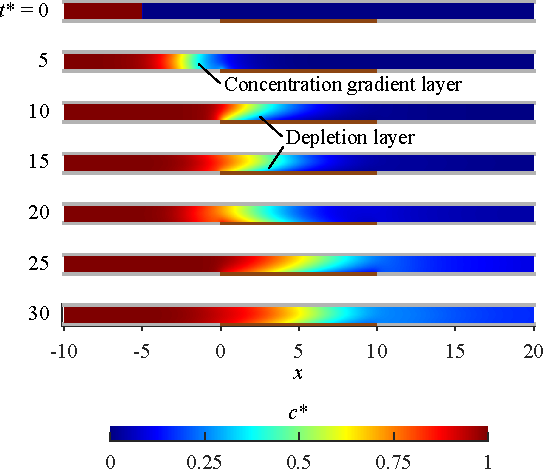
\includegraphics[width=0.45\textwidth]{figure/composite_case1_Pe1_10_Pe2_10.pdf}
  \caption{\color{blue}Evolution of the concentration field $c^*$ for case $A$ ($Pe_1 = Pe_2 = 10$). Other nondimensional parameters are listed in Table~\ref{tab:ABCD}. See supplementary movie for the evolution of $c^*$ at https://doi.org/xxx.xxx.}
  \label{fgr:concentrationA}
\end{figure}

{\color{blue}

We first present the computed temporal evolution of the distribution of concentration $c^*$ within the flow channel for four specific cases ($A$--$D$) from Group 1 in Table~\ref{tab:group}. As detailed in Table~\ref{tab:ABCD}, these cases share identical parameters for steady flow ($\lambda, Pe_1$) and adsorption kinetics ($\epsilon, Da, K_0$). For systematic comparison, cases $A$ and $B$ share the same oscillatory Péclet number $Pe_2$, while $A$ and $C$ share the same Womersley number $\alpha$. Similarly, $B$ and $D$ are characterized by the same $\alpha$, and $C$ and $D$ share the same $Pe_2$. Given $Pe_1 = 10$, the definition of the nondimensional time $t^*$ indicates that fluid particles originating from the channel inlet ($x = -5.0$) reach the leading edge of the reactive surface ($x = 0.0$) at $t^* \approx 5$ under the influence of the steady base flow. As $t^*$ evolves, distinct transport characteristics are observed across the four cases.

Case $A$, with $f = 1.0 \times 10^4$ and $a = 0.01$, represents the regime in which the steady and oscillatory Péclet numbers are comparable ($Pe_1 = 10$ and $Pe_2 = 10$). As seen in figure~\ref{fgr:concentrationA}, at $t^* = 0$, the concentration field is discontinuous in the streamwise direction: the injected solution occupies $-10 \leq x^* \leq -5$ with $c^* = 1$, whereas the downstream regime $-5 \leq x^* \leq 20$ initially has $c^* = 0$. By $t^* = 5$, the concentration front convected by the mean flow has reached the upstream edge of the reactive wall at $x^* = 0$. At this stage, the initially sharp concentration jump has already been smoothed by diffusion, so that a streamwise {\it concentration gradient layer} is established, i.e., the concentration now varies continuously along the $x^*$ direction instead of remaining sharply discontinuous \citep{Jiang_Zeng_Fu_Wu_2022, squires2008making}. In contrast, the wall-normal concentration gradient is still weak, indicating that transverse transport toward the reactive wall has not yet produced an evident near-wall low-concentration regime. At $t^* = 10$, the concentration contours become clearly inclined. This inclination reflects the combined effect of downstream advection-diffusion in the $x^*$ direction and transverse mass transport toward the reactive wall in the $y^*$ direction. Once adsorption over the range $0 \leq x^* \leq 10$ becomes appreciable, the concentration near the wall falls below that in the channel core, forming a locally depleted regime adjacent to the reactive wall, hereafter referred to as the {\it depletion layer} \citep{aquino2024equilibrium, wang2016solute}. Correspondingly, the wall-normal concentration gradient becomes pronounced, especially near the upstream part of the reactive segment where the concentration front first encounters the adsorbing surface. At $t^* = 15$, the concentration field is convected further downstream, and the inclined concentration front becomes more elongated in the streamwise direction. Meanwhile, the depletion layer is compressed toward the reactive wall, indicating a steeper wall-normal concentration gradient. These features suggest that, at this instant, the oscillatory flow reinforces the mean flow and enhances downstream transport. At $t^* = 20$, the oscillatory contribution reverses its direction and opposes the mean flow, so that the concentration field is pulled back upstream. The concentration contours are correspondingly shifted upstream, indicating a temporary retardation of the downstream propagation of the concentration front. Meanwhile, replenishment of solute from the bulk becomes less effective, and the depletion layer broadens, accompanied by a weaker wall-normal concentration gradient. At $t^* = 25$, the oscillatory effect is noticeably weakened, and the concentration field is again governed mainly by the mean flow. The concentration contours recover a downstream-oriented pattern, while the depletion layer remains present over the reactive wall. At this stage, however, its shape is controlled primarily by steady advection together with wall uptake, rather than by strong oscillatory modulation. By $t^* = 30$, the oscillatory flow again acts in the same direction as the mean flow, so that downstream transport is enhanced once more. The concentration front is further stretched downstream, whereas the depletion layer is compressed toward the wall. Consequently, the wall-normal concentration gradient increases again.

%For case $A$ with $f= 1.0 \times 10^4$ and $a=0.01$, ... initially at $t^* = 0.0$, as shown in figure~\ref{fgr:concentrationABC}($a$). {\color{red}(is $t^*=0.2$ in the figure correct? characteristics: gradient change in the depletion layer and the direction of the inclination)}


%{\color{brown}




%At $t^* = 15$, the concentration field is displaced further downstream, and the inclined concentration front becomes more elongated in the streamwise direction. Meanwhile, the near-wall low-concentration regime is compressed toward the reactive wall, indicating a thinner concentration boundary layer and a steeper wall-normal concentration gradient. These features suggest that, at this instant, the oscillatory flow reinforces the mean flow and enhances downstream transport. {\color{red}(need discussion)} As a result, the inclined concentration front is displaced further downstream and the concentration contours become more stretched in the streamwise direction. At the same time, the near-wall low-concentration regime becomes thinner, because fresh solute is brought more effectively from the bulk toward the reactive wall, which in turn steepens the wall-normal concentration gradient.

%At $t^* = 20$, the oscillatory contribution reverses its direction and opposes the mean flow, so that the concentration field is pulled back upstream. The concentration contours are correspondingly shifted upstream, indicating a temporary retardation of the downstream propagation of the concentration front. Meanwhile, replenishment of solute from the bulk becomes less effective, and the near-wall low-concentration regime broadens, accompanied by a weaker wall-normal concentration gradient.

%At $t^* = 25$, the oscillatory effect is noticeably weakened, and the concentration field is again governed mainly by the mean flow. The concentration contours recover a downstream-oriented pattern, while the near-wall low-concentration regime remains present over the reactive wall. At this stage, however, its shape is controlled primarily by steady advection together with wall uptake, rather than by strong oscillatory modulation.

%By $t^* = 30$, the oscillatory flow again acts in the same direction as the mean flow, so that downstream transport is enhanced once more. The concentration front is further stretched downstream, whereas the near-wall low-concentration regime is compressed toward the wall. Consequently, the wall-normal concentration gradient increases again.
%}

\begin{figure}
\centering
  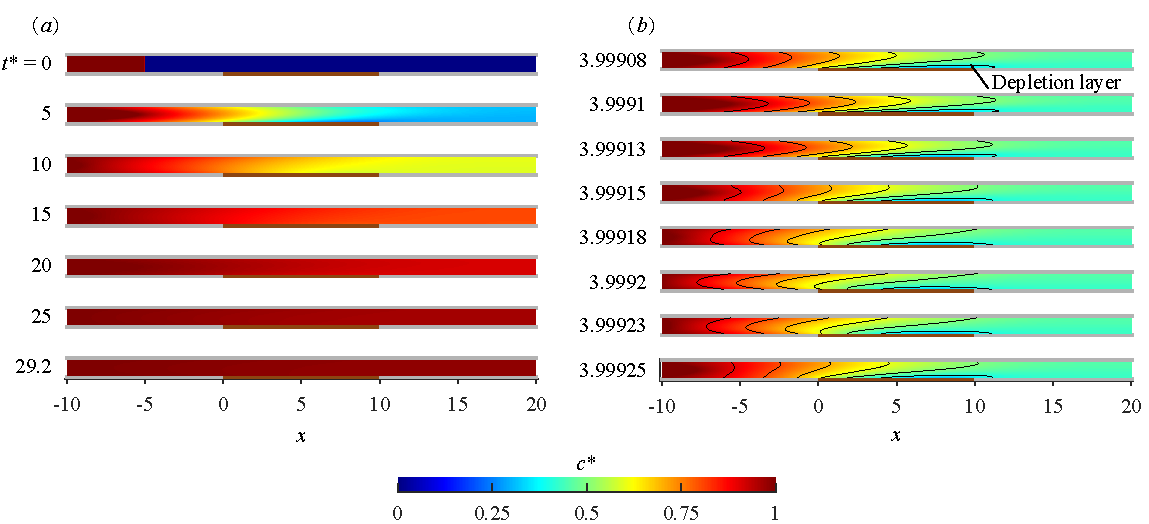
\includegraphics[width=0.95\textwidth]{figure/composite_case2_Pe1_10_Pe2_100000_v3.pdf}
  \caption{\color{blue}Evolution of the concentration field $c^*$ for case $B$ ($Pe_1 = 10,\, Pe_2 = 100000$). ($a$) Time-resolved plots over the full adsorption process, $0 \leq t^* \leq 29.2$. ($b$) Close-up view within one representative oscillation period of $3.99908 \leq t^* \leq 3.99925 \times 10^{-4}$, highlighting the oscillatory variation of the concentration field induced by the oscillating velocity field. Other nondimensional parameters are listed in table~\ref{tab:ABCD}. See supplementary movie for the evolution of $c^*$ at https://doi.org/xxx.xxx.}
  \label{fgr:concentrationB}
\end{figure}




For case $B$, with $f = 1.0 \times 10^4$ and $a = 1.0$, the oscillatory Péclet number is much larger than the steady Péclet number ($Pe_1 = 10$ and $Pe_2 = 100000$). As shown in figure~\ref{fgr:concentrationB}(a), the initial concentration field at $t^* = 0$ is the same as that in case $A$, with a sharp streamwise discontinuity between the upstream high-concentration regime and the downstream low-concentration regime. By $t^* = 5$, the concentration front has already propagated over most of the reactive section, and the initially sharp interface has evolved into a broad streamwise concentration gradient regime. A depletion layer is present adjacent to the reactive wall, but its wall-normal thickness is small compared with the streamwise spreading of the bulk concentration field. At $t^* = 10$, the concentration level over the reactive regime further increases, and the concentration contours become smoother along the channel. At $t^* = 15$ and $20$, the concentration field continues to approach a nearly saturated state, with only a weak streamwise variation remaining in the bulk regime. By $t^* = 25$ and $29.2$, the concentration field is almost fully developed over the computational domain. Compared with the weak oscillation case $C$, this rapid filling of the downstream regime indicates that the strong oscillatory transport substantially enhances the supply of solute to the reactive surface. The close-up temporal view in figure~\ref{fgr:concentrationB}$b$ further illustrates the intra-cycle behavior of the concentration field throughout one oscillation cycle. Although the overall concentration distribution remains nearly unchanged over this short interval, the concentration contours near the reactive wall exhibit an evident oscillatory displacement. The depletion layer remains attached to the reactive wall, but its shape and thickness vary periodically with the velocity field oscillation. When the oscillatory flow enhances downstream transport, the contours are stretched downstream and the depletion layer is compressed toward the wall. When the oscillatory contribution reverses, the contours are shifted upstream and the depletion layer broadens slightly. These features indicate that, in case $B$, the long-time adsorption process is strongly accelerated by the large oscillatory Péclet number, while the instantaneous concentration field retains a clear oscillatory signature near the reactive wall.

}

%The enlarged view in figure~\ref{fgr:concentrationB}(b) further reveals the intra-cycle response of the concentration field within one oscillation cycle. Although the overall concentration distribution remains nearly unchanged over this short interval, the concentration contours near the reactive wall exhibit an evident oscillatory displacement. The depletion layer remains attached to the reactive wall, but its shape and thickness vary periodically with the velocity field oscillation. When the oscillatory flow enhances downstream transport, the contours are stretched downstream and the depletion layer is compressed toward the wall. When the oscillatory contribution reverses, the contours are shifted upstream and the depletion layer broadens slightly. These features indicate that, in case $B$, the long-time adsorption process is strongly accelerated by the large oscillatory Péclet number, while the instantaneous concentration field retains a clear oscillatory signature near the reactive wall.

{\color{blue}
%For case $C$, where $Pe_1 \gg Pe_2$, the concentration field evolves in a manner very similar to that of the non-oscillatory case ($Pe_2 = 0$). {\color{magenta}(add $Pe_2=0$ case in appendix for comparison. and add references)} 
%At $t^* = 0$, the initial streamwise concentration discontinuity is the same as that in case A. 
%By $t^* = 5$, a depletion layer becomes evident adjacent to the reactive wall. At $t^* = 10$, the depletion layer broadens and extends further downstream, while the concentration contours become smoother in the streamwise direction. At $t^* = 15$, the concentration gradient layer is convected further downstream and becomes more diffuse. At $t^* = 20$, the depletion layer continues to develop, and the overall concentration field exhibits further axial spreading. At $t^* = 25$, the concentration profile continues to translate downstream while maintaining a smooth transition zone. By $t^* = 30$, the depletion layer remains clearly visible over an extended streamwise range. These features indicate that the oscillatory flow is too weak to produce an appreciable deviation from the steady-flow behaviour, consistent with the non-oscillatory results reported in \citet{Huang2023}. The characteristic adsorption timescale is likewise close to that of the steady-flow case, with the maximum adsorption rate occurring at approximately $t^* \approx 20$ and $99\%$ equilibrium reached at $t^*_{0.99,C} \approx 40$. {\color{magenta}(add figure ($b$) description and the reason for adding (for comparison with case D))}


For case $C$, where $Pe_1 \gg Pe_2$, the concentration field evolves in a manner very similar to that of the non-oscillatory case ($Pe_2 = 0$). {\color{magenta}(add $Pe_2=0$ case in appendix for comparison. and add references)}  As shown in figure~\ref{fgr:concentrationC}$a$, the overall evolution is dominated by the steady-flow transport. By $t^* = 5$, a depletion layer becomes evident adjacent to the reactive wall. At $t^* = 10$, the depletion layer broadens and extends further downstream, while the concentration contours become smoother in the streamwise direction. At $t^* = 15$, the concentration-gradient layer is convected further downstream and becomes more diffuse. At $t^* = 20$, the depletion layer continues to develop, and the overall concentration field exhibits further axial spreading. At $t^* = 25$, the concentration profile continues to translate downstream while maintaining a smooth transition zone. By $t^* = 30$, the depletion layer remains clearly visible over an extended streamwise range. Figure~\ref{fgr:concentrationC}$b$ provides a close-up temporal view of the early-time evolution over $0.1 \leq t^* \leq 0.7$. During this interval, the concentration-gradient layer remains close to the initial interface and advances only gradually downstream. The contours are slightly inclined but show no evident oscillatory displacement, indicating that the weak oscillatory component has little influence on the early development of the concentration field. This close-up view is included to provide a reference for comparison with case $D$, where the stronger oscillatory transport produces a more visible modulation of the early-time concentration-gradient layer. These features indicate that the oscillatory flow is too weak to produce an appreciable deviation from the steady-flow behaviour, consistent with the non-oscillatory results reported in \citet{Huang2023}.

For case $D$, the oscillatory Péclet number is larger than that in case $C$ but remains smaller than the strongly oscillatory case $B$. As shown in figure~\ref{fgr:concentrationD}$a$, the overall evolution of the concentration field is still mainly characterized by downstream propagation of the concentration front. By $t^* = 5$, a depletion layer becomes visible adjacent to the reactive wall. At $t^* = 10$, the depletion layer broadens and the concentration gradients become more inclined near the upstream part of the reactive segment. At $t^* = 15$ and $20$, the concentration-gradient layer is convected further downstream and becomes more diffuse. At $t^* = 25$, the concentration profile continues to translate downstream while maintaining a smooth transition zone. By $t^* = 30$, the depletion layer remains present over the reactive wall, and the concentration field shows a broader downstream spreading than in the earlier stages. Figure~\ref{fgr:concentrationD}$b$ shows the early-time evolution over $0.1 \leq t^* \leq 0.7$. Compared with case $C$, the concentration-gradient layer is clearly broadened in the streamwise direction. The concentration contours spread over a wider range of $x^*$, indicating that the oscillatory flow enhances transport alternately in the positive and negative streamwise directions. This repeated forward-and-backward motion stretches the initially sharp concentration front and increases the streamwise thickness of the gradient layer. These features suggest that the oscillatory component has begun to affect the local concentration structure, although it is still not strong enough to dominate the overall adsorption process. These features suggest that case $D$ represents an intermediate response between the weak-oscillation behaviour in case $C$ and the strongly oscillatory behaviour in case $B$. The mean downstream transport remains important, but the oscillatory flow already produces a detectable modulation of the early-time concentration-gradient layer.




\begin{figure}
\centering
  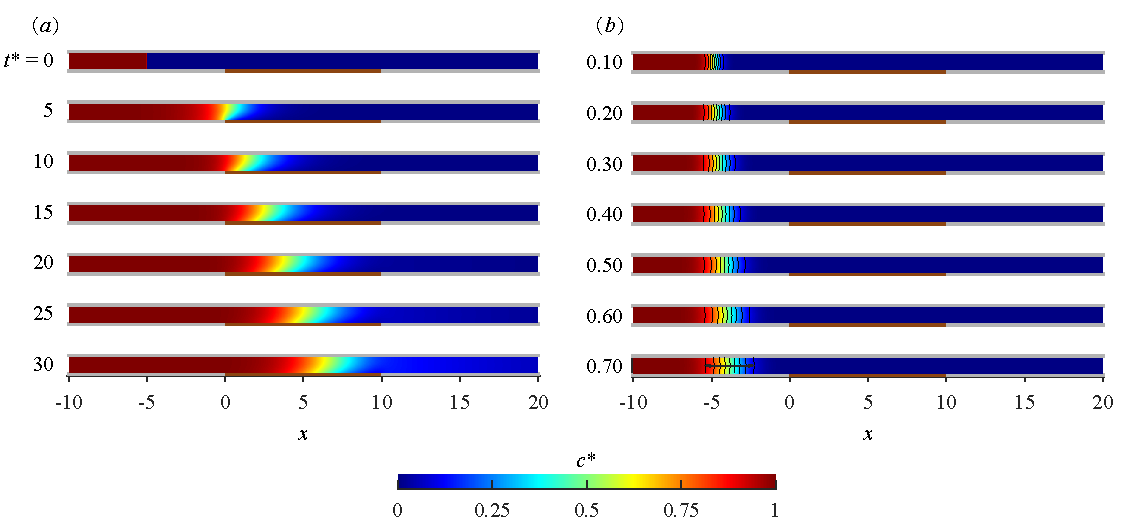
\includegraphics[width=0.95\textwidth]{figure/composite_case3_Pe1_10_Pe2_0.01_v3.pdf}
  \caption{\color{blue}Evolution of the concentration field $c^*$ for case $C$ ($Pe_1 = 10,\, Pe_2 = 0.01$). ($a$) Time-resolved plots over the selected adsorption process, $0 \leq t^* \leq 30$. ($b$) Close-up view over $0.1 \leq t^* \leq 0.7$, showing the temporal development of the concentration gradient layer. Other nondimensional parameters are listed in table~\ref{tab:ABCD}. See supplementary movie for the evolution of $c^*$ at https://doi.org/xxx.xxx. }
  \label{fgr:concentrationC}
\end{figure}

\begin{figure}
\centering
  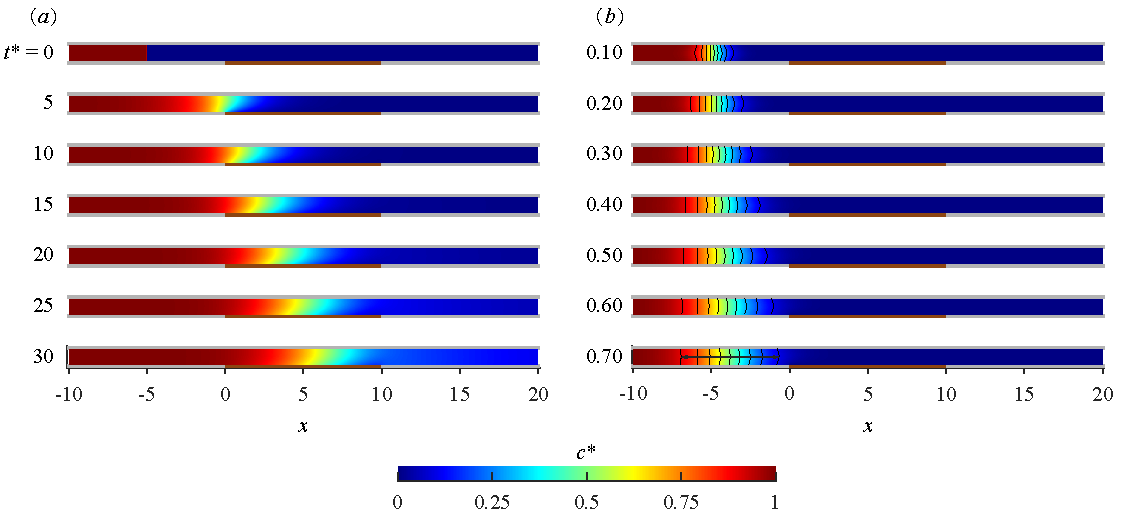
\includegraphics[width=0.95\textwidth]{figure/composite_case4_Pe1_10_Pe2_1000_v3.pdf}
  \caption{\color{blue}Evolution of the concentration field $c^*$ for case $D$ ($Pe_1 = 10,\, Pe_2 = 1000$). ($a$) Time-resolved plots over the selected adsorption process, $0 \leq t^* \leq 30$. ($b$) Close-up view over $0.1 \leq t^* \leq 0.7$, showing the temporal development of the concentration gradient layer. Other nondimensional parameters are listed in table~\ref{tab:ABCD}. See supplementary movie for the evolution of $c^*$ at https://doi.org/xxx.xxx.}
  \label{fgr:concentrationD}
\end{figure}

%In Fig.~\ref{fgr:concentrationABC}, we present the computed temporal evolution of the concentration distribution $c^*$ within the flow channel for four specific cases ($A, B, C$, and $D$) from Group 1 in Table~\ref{tab:group}. As detailed in Table~\ref{tab:ABCD}, these cases share identical steady-flow parameters ($\lambda, Pe_1$) and adsorption kinetics ($\epsilon, Da, K_0$). For systematic comparison, cases $A$ and $B$ share the same oscillatory Péclet number $Pe_2$, while $A$ and $C$ share the same Womersley number $\alpha$. Similarly, $B$ and $D$ are characterized by the same $\alpha$, and $C$ and $D$ share the same $Pe_2$. Given $Pe_1 = 10$, the definition of nondimensional time $t^*$ indicates that fluid particles originating from the channel inlet ($x = 5$) reach the leading edge of the reactive surface ($x = 10$) at $t^* \approx 5.2$ under the influence of the steady base flow.As $t^*$ evolves, distinct transport characteristics are observed across the four cases. 

% Case $A$ exhibits a pronounced concentration depletion zone near the reactive surface throughout the simulation, where the concentration of free adsorbates decreases significantly. In this regime, the adsorbates bind to the surface at a rate exceeding the diffusive supply from the bulk flow \cite{Huang2023}. A unique feature of Case $A$ is the discernible influence of $Pe_2$; the boundary slope of the depletion zone periodically reverses, closely following the alternating direction of the oscillatory flow.In contrast, cases $B, C$, and $D$ do not exhibit such slope reversals at the depletion zone boundary. In these instances, the impact of the reciprocating flow on the concentration gradient appears negligible, resulting in concentration profiles that closely resemble classical steady flow results. This behavior is physically consistent for cases $B$ and $C$, where the transport is dominated by a single Péclet number ($Pe_1 \ll Pe_2$ for $B$ or $Pe_1 \gg Pe_2$ for $C$), thereby adhering to the steady flow limits established in previous studies. Surprisingly, Case $D$ maintains a depletion zone thickness that does not contract despite the high-frequency oscillations (large $\alpha$) and the associated thinning of the oscillatory boundary layer. Consequently, Case $D$ behaves much like a steady-flow system. Its concentration field distribution differs significantly from Case $A$ but shows high similarity to Case $C$, with the primary distinction being a slight apparent delay in the flow response.

\begin{figure}
    \centering
    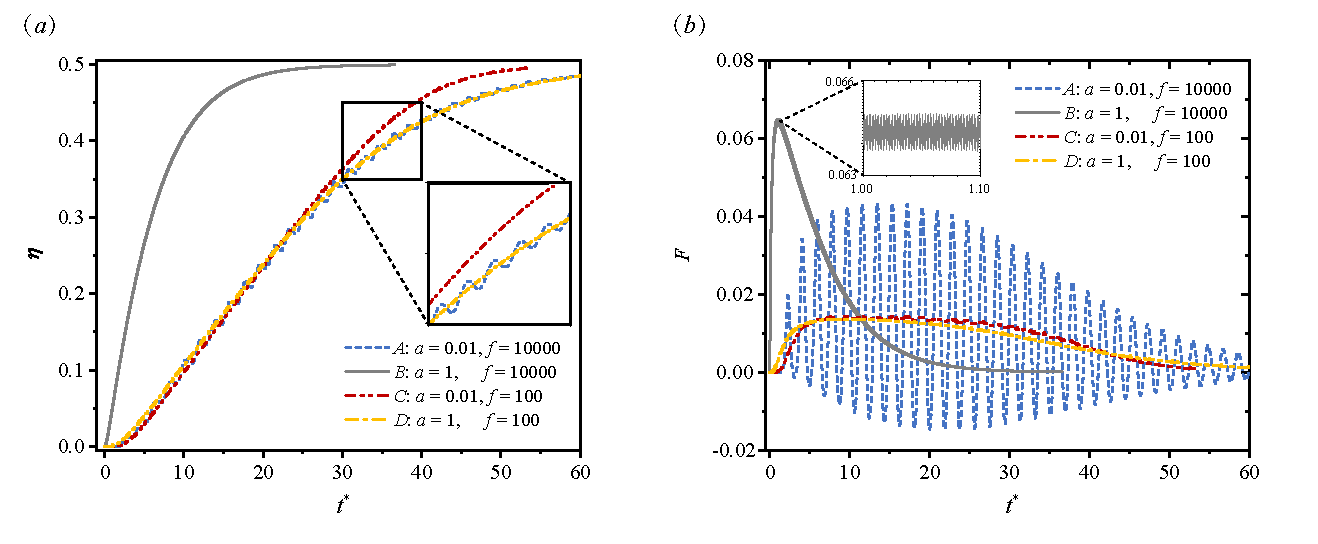
\includegraphics[width=\textwidth]{figure/eta_ave_ABCD_v6.pdf}
    \caption{Evolution of ($a$) $\eta_{\rm ave}$ and ($b$) $ {F}_{\rm ave}$ over time $t^*$ for cases $A$--$D$, whose values of nondimensional parameters are listed in Table ~\ref{tab:ABCD}. 
   % {\color{magenta}(add (a) and (b) in the figure. change curve color and style (too thin). case D? note the font difference between text and figure. add t0.99 identification in the figure.)}
    }
    \label{fig:eta_ave_ABCD}
\end{figure}

Figure~\ref{fig:eta_ave_ABCD} compares the adsorption dynamics of cases $A$--$D$ using the temporal evolution of the spatially averaged surface concentration $\eta_{\rm ave}$, and the averaged dimensionless adsorption flux $F$. The two quantities provide complementary information: $\eta_{\rm ave}$ describes the cumulative adsorption process, whereas $F$ reflects the instantaneous rate at which solute is supplied to and captured by the reactive surface.
As shown in figure~\ref{fig:eta_ave_ABCD}$a$, $\eta_{\rm ave}$ increases monotonically in all four cases and gradually approaches its equilibrium value. The curves, however, differ substantially in their growth rates. Case $B$ reaches the equilibrium much earlier than the other cases, indicating a rapid supply of solute to the reactive surface under the strong oscillatory flow. Cases $A$, $C$ and $D$ evolve more slowly and remain close to each other over most of the adsorption process.
The flux histories in figure~\ref{fig:eta_ave_ABCD}$b$ reveal more detailed differences among the four cases. In case $B$, the adsorption flux rises rapidly to a large early-time peak and then decays quickly as the surface concentration approaches equilibrium. This behaviour is consistent with the fast saturation observed in figure~\ref{fig:eta_ave_ABCD}$a$. In case $C$, the flux varies smoothly and exhibits no evident oscillatory modulation, consistent with the weak-oscillation limit in which the transport process is close to the non-oscillatory case.

Cases $A$ and $D$ show a different type of response. In case $A$, the flux exhibits pronounced high-frequency oscillations, indicating that the wall adsorption rate is directly modulated by the imposed oscillatory flow. The oscillations decay gradually as the adsorption process approaches equilibrium. In contrast, case $D$ displays a much smoother flux curve, but its overall evolution is closer to case $A$ than to case $C$. The corresponding $\eta_{\rm ave}(t^*)$ curve may be viewed as a smoothed version of the case $A$ response: the high-frequency oscillations are filtered out, while the underlying adsorption trend remains similar.



This comparison shows that the evolution of the concentration field alone does not fully determine the adsorption kinetics. Although cases $C$ and $D$ have visually similar downstream development of the concentration field, their $\eta_{\rm ave}$ and $F$ histories indicate different dynamical responses. In contrast, cases $A$ and $D$ share similar adsorption trends even though their instantaneous flux oscillations differ markedly. These observations motivate the parameter-space analysis in the next section, where the combined effects of oscillation frequency and amplitude are examined systematically through the averaged adsorption flux $F_{\rm ave}$ and the corresponding enhancement factor.
{\color{green}here}

}

\section{Phase diagrams of the time-averaged adsorption flux}
\label{sec:phase_diagrams}

The systematic parameter sweep summarized in Table~\ref{tab:group} gives
the time-averaged adsorption flux $F_{\rm ave}$ over the $(f,a)$ plane
for each prescribed value of $Pe_1$. Here $f$ and $a$ denote the
dimensionless oscillation frequency and amplitude, respectively. Their
relations to the oscillatory parameters $(\alpha,Pe_2)$ are given in
Appendix~\ref{appdix-D}. Figure~\ref{fig:phase_diagram} shows representative
phase diagrams for $Pe_1=10$ and $Pe_1=100$.

For each point in the $(f,a)$ plane, the saturation time $t_{0.99}^*$ is
extracted from the temporal evolution of the spatially averaged surface
concentration $\eta_{\rm ave}(t^*)$, following Eq.~\eqref{eq:saturation_time}.
The time-averaged adsorption flux is then calculated as
$F_{\rm ave}=\eta_{\rm eq}/t_{0.99}^*$ according to Eq.~\eqref{eq:Fave}.
The resulting scalar field $F_{\rm ave}(f,a)$ is plotted using a logarithmic
colour scale, and black contour lines are superimposed to indicate the
variation of the adsorption flux across the parameter space.

To evaluate the effect of oscillation relative to the steady-flow baseline,
we define the adsorption-enhancement factor
\begin{equation}
\mathcal{E}(f,a) =
\frac{F_{\rm ave}(f,a;Pe_1)}
{F_{\rm ave}^{(0)}(Pe_1)},
\label{eq:enhancement_factor}
\end{equation}
where $F_{\rm ave}^{(0)}$ is the value obtained for the non-oscillatory
case at the same $Pe_1$. Thus, $\mathcal{E}>1$ indicates that the imposed
oscillation enhances the overall adsorption rate, whereas $\mathcal{E}<1$
indicates a reduction relative to the steady-flow case. The value
$\mathcal{E}\approx 1$ corresponds to a response that is nearly unchanged
by the oscillatory component.

As shown in Fig.~\ref{fig:phase_diagram}, the response in the $(f,a)$ plane
can be divided into three main regimes. At low values of both $f$ and $a$,
the contours of $F_{\rm ave}$ are weakly affected by the oscillatory forcing,
and the enhancement factor remains close to unity. This regime is therefore
identified as regime~I, where the adsorption process is controlled mainly
by the steady flow. In this regime, the behaviour is expected to recover the
steady-flow scaling discussed in our previous work \citep{Huang2024}.

At large values of $f$ and $a$, the adsorption flux increases markedly
compared with the steady-flow baseline. The enhancement factor becomes
much larger than unity, indicating that the oscillatory component provides
the dominant contribution to solute transport toward the reactive surface.
This regime is denoted as regime~III. In the following analysis, the data in
this regime are examined in terms of an effective oscillatory Péclet number,
in order to test whether the response can be collapsed onto a common
scaling independent of $Pe_1$.

Between regimes~I and III, the contour pattern changes rapidly with both
$f$ and $a$. In this intermediate range, the adsorption flux cannot be
described solely by the steady Péclet number $Pe_1$ or by the oscillatory
Péclet number $Pe_2$. The corresponding time histories of
$\eta_{\rm ave}(t^*)$ also show clear oscillatory modulation, as illustrated
later in Fig.~\ref{fig:eta_ave_ABCD}. This intermediate part of the phase
diagram is referred to as regime~II. It represents the regime in which the
oscillatory forcing and the surface adsorption process interact most strongly.

A narrow band is observed between regime~II and regime~III. In this band,
the inferred value of $F_{\rm ave}$ is sensitive to the saturation threshold
used in the definition of $t_{0.99}^*$. This sensitivity occurs because
$\eta_{\rm ave}(t^*)$ approaches $\eta_{\rm eq}$ slowly at late times; as a
result, changing the threshold from $0.99$ to $0.95$ can shift the apparent
location of the boundary. Since this band reflects the operational definition
of the saturation time rather than a separate transport mechanism, it is not
treated as an additional fundamental regime. The threshold sensitivity is
examined separately in Appendix~\ref{appdix-B}.

Table~\ref{tab:regime_summary} summarizes the three main regimes identified
from the phase diagrams. regimes~I and III correspond to two limiting
behaviours, controlled primarily by the steady flow and the oscillatory
transport, respectively. regime~II connects these two limits and contains
the strongest dependence on both $f$ and $a$. The following sections first
analyse the limiting behaviour in regimes~I and III, and then discuss the
mechanism responsible for the intermediate response in regime~II.

\begin{table}
\begin{center}
\def~{\hphantom{0}}
\begin{tabular*}{\textwidth}{@{\extracolsep{\fill}} l l l l}
\hline
Regime & Location in $(f,a)$ & Main feature & Dominant effect \\
\hline\\[-6pt]
regime~I
& Low $f$, low $a$
& $\mathcal{E}\approx 1$
& Steady-flow controlled \\[4pt]

regime~II
& Intermediate $f$ and $a$
& Strong variation of $F_{\rm ave}$
& Coupled oscillatory transport and adsorption \\[4pt]

regime~III
& High $f$, high $a$
& $\mathcal{E}\gg 1$
& Oscillation-dominated transport \\
\hline
\end{tabular*}
\caption{Summary of the three main regimes observed in the $(f,a)$ phase
diagram. The enhancement factor $\mathcal{E}$ is defined in
Eq.~\eqref{eq:enhancement_factor}.}
\label{tab:regime_summary}
\end{center}
\end{table}

\begin{figure}
    \centering
    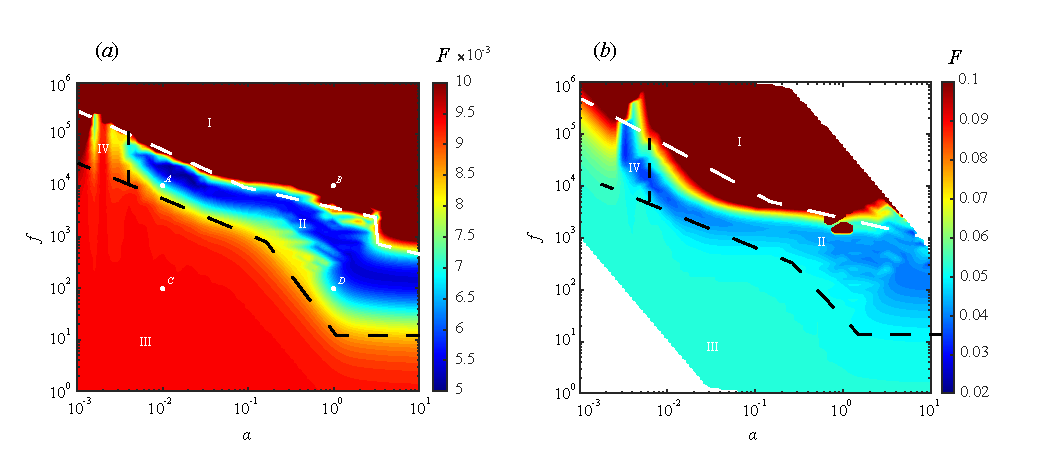
\includegraphics[width=1\textwidth]{figure/contour_plot_v6.pdf}
    \caption{Phase diagram of average adsorption flux $F_{\rm ave}$ as a function of the dimensionless frequency $f$ and amplitude $a$. The diagram is divided into three characteristic regimes as discussed in the text.((a) a weak steady base flow ($Pe_1 = 10$) and (b) a strong steady base flow ($Pe_1 = 100$)) {\color{red}(what do the black curves stand for? label font size too small. indicate three regimes)}}
    \label{fig:phase_diagram}
\end{figure}

\subsection{Steady-flow equivalence in regimes~I and III}
\label{sec:regimes_I_III}
 
Sections~\ref{sec:regime_identification} introduced three principal
regimes in the $(f,\, a)$ phase diagram. Two of them, regime~I and
regime~III, are characterised by an essentially steady-flow response of
the time-averaged adsorption flux: although the underlying flow field is
unsteady, the long-time-averaged transport reduces to that of an
equivalent steady Poiseuille flow, with only the controlling P\'{e}clet
number differing between the two regimes. This section establishes that
equivalence quantitatively. We first recall the steady-flow scaling law
that serves as the reference baseline (Section~\ref{sec:steady_recap}),
then show that regime~I is a small-amplitude perturbation of the steady
problem (Section~\ref{sec:regime_I_scaling}), and finally demonstrate
that regime~III admits a single-parameter collapse onto an effective
steady-flow law characterised by an $\alpha$-modified oscillatory
P\'{e}clet number (Section~\ref{sec:regime_III_scaling}).
 
%------------------------------------------------------------------
\subsubsection{Reference: steady-flow scaling of the adsorption flux}
\label{sec:steady_recap}
 
In the absence of oscillation ($Pe_2 = 0$), the time-averaged adsorption
flux $F_{\rm ave}^{(0)}$ is governed by the classical
advection--diffusion balance in a plane Poiseuille flow with a reactive
wall. Following the analysis in our previous work \citep{Huang2024},
the steady-flow flux exhibits a L\'{e}veque-type scaling in the
high-P\'{e}clet limit,
\begin{equation}
F_{\rm ave}^{(0)} \;\sim\; C_{0}(Da,\,\epsilon,\,K_{0})\; Pe_{1}^{\,n_{0}},
\label{eq:steady_scaling}
\end{equation}
where the exponent $n_{0}$ approaches $1/3$ in the diffusion-limited
boundary-layer regime and the prefactor $C_{0}$ encodes the influence of
the surface kinetics parameters. The exact form of $C_{0}$ and the
crossover from reaction-limited to transport-limited behaviour at
moderate $Pe_{1}$ is documented in Appendix~\ref{appdix-C}.
{(fill in numerical values of $n_{0}$ and the prefactor extracted from current data; verify consistency with Huang 2024)}
Equation~\eqref{eq:steady_scaling} provides the baseline against which
all oscillatory results in this study are compared.
 
%------------------------------------------------------------------
\subsubsection{regime~I as a small-amplitude perturbation}
\label{sec:regime_I_scaling}
 
In regime~I, the oscillatory P\'{e}clet number is much smaller than its
steady counterpart, $Pe_{2} \ll Pe_{1}$, and the dimensionless amplitude
$a$ is sufficiently small that the oscillatory velocity component can be
treated as a perturbation of the mean Poiseuille profile. A formal
linearization in $Pe_{2}/Pe_{1}$ predicts that the leading-order
correction to the time-averaged flux is of order
$(Pe_{2}/Pe_{1})^{2}$, since the contribution linear in the oscillation
amplitude averages to zero over one period. Consequently, the
enhancement factor satisfies
\begin{equation}
\mathcal{E}(f,\, a;\, Pe_{1}) \;=\; 1 \;+\; \mathcal{O}\!\left(
\frac{Pe_{2}^{\,2}}{Pe_{1}^{\,2}} \right)
\quad\text{in regime~I.}
\label{eq:regime_I_perturbation}
\end{equation}
 
Figure~\ref{fig:regime_I_collapse} (\textit{a}) tests this prediction by
plotting $\mathcal{E} - 1$ as a function of $Pe_{2}/Pe_{1}$ for several
fixed values of $\alpha$ within regime~I. The data collapse onto a
single quadratic envelope, confirming that the oscillation contributes
only a small, sign-indefinite correction to the steady-flow flux in this
regime. The boundary of regime~I, defined operationally by
$|\mathcal{E} - 1| = \delta_{\rm I}$ with $\delta_{\rm I} = 0.05$
(Section~\ref{sec:regime_identification}), corresponds to a critical
ratio $(Pe_{2}/Pe_{1})_{\rm cr}$ that depends weakly on $\alpha$.
{(insert numerical value of the critical ratio once
extracted; create Fig.~\ref{fig:regime_I_collapse})}
 
The practical implication of Eq.~\eqref{eq:regime_I_perturbation} is
that, throughout regime~I, the design of an oscillatory ADR system can
proceed by direct use of the steady-flow expressions in
\citep{Huang2024} without explicit treatment of the unsteady
contribution. The role of regime~I in the present study is thus to
serve as a consistency check on the numerical methodology and to
delineate the parameter range in which oscillatory effects can safely
be ignored.
 
%------------------------------------------------------------------
\subsubsection{regime~III: $\alpha$-modified oscillatory P\'{e}clet number}
\label{sec:regime_III_scaling}
 
The situation in regime~III is qualitatively different. Here the
oscillatory amplitude dominates the steady mean flow,
$Pe_{2} \gg Pe_{1}$, and the time-averaged transport is governed by the
oscillatory component alone. Naively one might expect $F_{\rm ave}$ in
this regime to scale as a function of $Pe_{2}$ alone, by direct analogy
with the steady-flow result of Eq.~\eqref{eq:steady_scaling}. However,
because the spatial structure of the oscillatory velocity profile
depends strongly on the Womersley number $\alpha$
(figure~\ref{fig:f_a_1}), the effective rate of mass transport between
the bulk and the reactive wall is not simply set by the amplitude
$Pe_{2}$, but rather by the product of the amplitude and an
$\alpha$-dependent geometric factor.
 
Motivated by this observation, we test a collapse of the form
\begin{equation}
F_{\rm ave}(f,\, a;\, Pe_{1}) \;=\; \mathcal{F}\!\left( Pe_{\rm eff} \right),
\qquad
Pe_{\rm eff} \;\equiv\; Pe_{2}\; g(\alpha),
\label{eq:regime_III_collapse}
\end{equation}
where $\mathcal{F}$ is a universal function recovering the steady-flow
scaling of Eq.~\eqref{eq:steady_scaling} when $Pe_{\rm eff} \to Pe_{1}$,
and $g(\alpha)$ is a dimensionless geometric weight to be determined
from the data. Two limiting forms of $g(\alpha)$ are physically
anticipated. In the low-frequency limit, the oscillatory profile reduces
to a quasi-steady Poiseuille shape, so that
$g(\alpha) \to 1$ for $\alpha \to 0$. In the high-frequency limit, the
oscillatory motion is confined to a thin Stokes layer of thickness
$\delta_{\rm S}/H \sim 1/\alpha$ near the wall, and the effective shear
rate seen by the concentration boundary layer scales as $\alpha$; this
suggests $g(\alpha) \sim \alpha^{p}$ with $0 < p \le 1$ at large
$\alpha$.
 
Figure~\ref{fig:regime_III_collapse} reports the empirical collapse
obtained from the present simulations. Within regime~III, all data
falling above the operational threshold collapse onto a single master
curve when plotted against $Pe_{\rm eff}$, with the form of $g(\alpha)$
determined by a least-squares fit to be
\begin{equation}
g(\alpha) \;=\; ??\,,
\label{eq:g_alpha_fit}
\end{equation}
{(insert fitted functional form and the corresponding
exponent $p$ once extracted; suggested fit family:
$g(\alpha) = (1+(\alpha/\alpha_{*})^{p})^{q}$)}
which interpolates smoothly between the two limiting behaviours
discussed above. The corresponding collapse is shown in
Figure~\ref{fig:regime_III_collapse} (\textit{b}); the relative scatter
of the data around the master curve is below \textit{??}\,\%, supporting
the view that regime~III is, to a good approximation, a steady-flow
problem with the controlling P\'{e}clet number $Pe_{\rm eff}$ replacing
$Pe_{1}$.
 
The two limiting cases of practical interest are recovered immediately.
For $\alpha \to 0$, the system behaves as a steady Poiseuille flow
driven by the time-averaged oscillatory pressure gradient; for
$\alpha \gg 1$, the high-frequency Stokes layer transports mass to the
wall at a rate proportional to $\alpha^{p} Pe_{2}$, providing a simple
design rule for the enhancement achievable by high-frequency
forcing.
 
%------------------------------------------------------------------
\subsubsection{Transition to the genuinely unsteady regime}
\label{sec:transition_to_regimeII}
 
The analysis above shows that the two outer regimes of the phase
diagram are reducible to steady-flow problems, differing only in
whether the controlling P\'{e}clet number is $Pe_{1}$ (regime~I) or
$Pe_{\rm eff}(Pe_{2},\,\alpha)$ (regime~III). The intermediate
regime~II, by contrast, cannot be brought into this form: as will be
shown in Section~\ref{sec:regime_II_mechanism}, the time-averaged
adsorption flux there depends on the oscillation frequency through a
genuinely dynamical mechanism --- the finite response time of the
surface Langmuir kinetics --- which has no counterpart in any
steady-flow problem. The next section is devoted to this mechanism.

\subsection{Oscillation-driven mechanisms in regime II}

\subsection{Influence of the steady Péclet number on the phase diagram}

\section{Conclusions}
\label{sec:5}

In this work, we developed a numerical framework for simulating advection--diffusion--reaction transport under pulsatile flow conditions and conducted a comprehensive parametric study spanning 26,244 simulation cases across four steady P\'{e}clet numbers $Pe_1$.

The main findings are summarised as follows:
\begin{enumerate}
    \item A phase diagram of the average adsorption flux $F_{\rm ave}$ in the $(f,\,a)$ parameter space reveals three distinct transport regimes. In the $Pe_1$-dominated regime (regime~I) and the $Pe_2$-dominated regime (regime~III), the adsorption characteristics remain governed by an effective steady-flow description, consistent with the scaling framework established in~\citep{Huang2024}. In the transitional regime (regime~II), the adsorption process exhibits pronounced oscillatory behaviour that cannot be reduced to a steady-flow analogy.

    \item {\color{green}Second key finding, e.g.\ resonance structure, ridge-like feature in the phase diagram, or identification of optimal operating conditions.}

    \item {\color{green}Third key finding, e.g.\ scaling law for regime boundaries, critical transition criteria, or engineering design guidelines.}
\end{enumerate}

These results provide a unified picture of how pulsatile flow modulates surface adsorption across a broad range of operating conditions. The identified regime boundaries offer practical guidelines for selecting optimal frequency and amplitude combinations to enhance or control adsorption performance in applications such as {\color{green}specific application scenarios}.

Future work may extend the present framework to {\color{green}possible extensions, e.g.\ three-dimensional geometries, nonlinear reaction kinetics, or turbulent pulsatile flows}.


\backsection[Acknowledgements]{We gratefully acknowledge ...}

\backsection[Funding]{This study was supported by the National Natural Science Foundation of China (Grant U24A20140). H. Hua was supported by the Science and Technology Innovation 2030 (2023ZD0120604) and Basic Research Projects of Key Scientific Research Projects Plan in Henan Higher Education Institutions (25ZX013).}

\backsection[Declaration of interests]{The authors report no conflict of interest.}

\backsection[Author ORCIDs]{
\\Bo Huang, https://orcid.org/0000-0002-6517-4939;
\\Haobo Hua, https://orcid.org/0000-0002-8015-6392;
\\Shuhong Liu, https://orcid.org/0000-0003-2525-2303;
\\Zhigang Zuo, https://orcid.org/0000-0002-7407-0904.
}


\appendix

\section{Validation of numerical schemes and benchmarking}
\label{appdix-A}
 
This appendix documents the verification of the finite-difference solver
described in Section~\ref{sec:2}. Four complementary tests are
presented. Section~\ref{sec:appA_benchmark} compares the present solver
against published analytical and numerical results for advection--
diffusion--reaction (ADR) transport in steady and pulsatile flows.
Section~\ref{sec:appA_grid} reports a systematic spatial convergence
study, in which the time-averaged adsorption flux $F_{\rm ave}$ is
extracted at successively refined grids and the asymptotic value is
estimated by Richardson extrapolation. Section~\ref{sec:appA_time}
documents the temporal convergence of the explicit time-marching scheme
under both the Courant--Friedrichs--Lewy (CFL) stability constraint and
the oscillation-resolution constraint introduced in
Eq.~\eqref{eq:dt_oscillation}. Finally, Section~\ref{sec:appA_range}
delineates the parameter range over which the present results are
quantitatively reliable and identifies the regimes of the
$(Pe_{1},\,Pe_{2},\,\alpha,\,Sc)$ parameter space that require
specialised multiscale techniques beyond the scope of this study.
 
%------------------------------------------------------------------
\subsection{Comparison with published benchmark solutions}
\label{sec:appA_benchmark}
 
Three independent benchmark cases are used to verify the present solver
against established results.
 
\medskip
\noindent\textit{(i) Steady Poiseuille flow with first-order surface
reaction (Huang \textit{et al.} 2023).}
The first benchmark sets $Pe_{2} = 0$ and recovers the steady plane
Poiseuille configuration studied in our previous work
\citep{Huang2023}. The time-averaged adsorption flux $F_{\rm ave}$ and
the saturation time $t_{0.99}^{*}$ are computed for the parameter
combinations reported in Table~\textit{??} of \citep{Huang2023} and
compared with the corresponding values from that work. The relative
discrepancy in $F_{\rm ave}$ is below \textit{??\,\%} across all tested
cases, confirming that the present implementation correctly reduces to
the steady-flow limit. {\color{magenta}(insert numerical comparison
table; suggested format: $Pe_{1}$, $Da$, $\epsilon$, $K_{0}$,
$F_{\rm ave}^{\rm present}$, $F_{\rm ave}^{\rm Huang2023}$, relative
error)}
 
\medskip
\noindent\textit{(ii) Oscillatory Womersley flow without surface
reaction.}
The second benchmark suppresses the surface reaction
($Da \to 0$, $b_{\max} \to \infty$) and compares the computed velocity
field with the analytical Womersley solution for a plane oscillatory
flow at several values of $\alpha$
(figure~\ref{fig:f_a_1}). The velocity profiles at the four
representative phases discussed in Section~\ref{sec:2} agree with the
analytical expressions of \cite{ma2017theoretical} to within
\textit{??\,\%} in the $L^{2}$ norm. This test verifies the correct
discretisation of the time-dependent advection term and the proper
implementation of the no-slip boundary condition at the channel walls.
 
\medskip
\noindent\textit{(iii) Pulsatile dispersion with linear wall kinetics
(Mazumder \& Das 1992).}
The third benchmark compares the solute concentration distribution and
the longitudinal dispersion coefficient with the numerical results of
\cite{mazumder1992effect} for pulsatile flow in a channel with
first-order wall reaction. The parameter combinations are chosen to
match the linearised limit of the Langmuir model used in the present
work ($K_{0} \to \infty$, so that the desorption term is negligible
and the surface kinetics reduce to first-order adsorption). The
agreement in the cross-sectionally averaged concentration profile is
within \textit{??\,\%} at the time horizons reported in
\citep{mazumder1992effect}. {\color{magenta}(complete the comparison
once the Mazumder reproduction case is run; this is the most important
external benchmark for the oscillatory part of the solver)}
 
%------------------------------------------------------------------
\subsection{Spatial grid convergence}
\label{sec:appA_grid}
 
The sensitivity of the computed adsorption flux to the spatial
resolution is assessed for two representative cases that bracket the
range of difficulty encountered in the parameter sweep of
Table~\ref{tab:group}.
 
\medskip
\noindent\textit{Case G1 (mild regime).}
A representative case in regime~I with $Pe_{1} = 100$, $Pe_{2} = 10$,
$\alpha = 1$, and $Sc = 1000$ is run on four uniform grids with
$N_{y} = 50$, $100$, $150$, and $200$, keeping the aspect ratio
$h = L'/N_{x} = H/N_{y}$ fixed. The time-averaged adsorption flux
$F_{\rm ave}$ varies by less than \textit{??\,\%} between $N_{y} = 100$
and $N_{y} = 200$, indicating that $N_{y} = 100$ is already in the
asymptotic convergence range for this parameter combination.
 
\medskip
\noindent\textit{Case G2 (challenging regime).}
A representative case in regime~II with $Pe_{1} = 10$, $Pe_{2} = 10^{4}$,
$\alpha = 5$, and $Sc = 16000$ is run on the same four grids. The
extracted $F_{\rm ave}$ exhibits a stronger dependence on $N_{y}$ in
this case: the relative variation between $N_{y} = 100$ and
$N_{y} = 200$ is \textit{??\,\%}, decreasing to \textit{??\,\%} between
$N_{y} = 150$ and $N_{y} = 200$. The dependence is consistent with a
second-order Richardson extrapolation, yielding an estimated grid-
independent value $F_{\rm ave}^{\infty} = $ \textit{??}, which differs
from the $N_{y} = 150$ result used in the production sweep by
\textit{??\,\%}.
 
The origin of the stronger grid sensitivity at large $\alpha$ and
$Sc$ is the increasingly thin concentration boundary layer at the
reactive wall, whose characteristic thickness scales as
\begin{equation}
\frac{\delta_{c}}{H} \;\sim\; \frac{1}{\alpha \sqrt{Sc}}\,.
\label{eq:bl_thickness}
\end{equation}
For Case G2, Eq.~\eqref{eq:bl_thickness} predicts
$\delta_{c}/H \sim 1.6 \times 10^{-3}$, so that a uniform grid with
$N_{y} = 150$ places \textit{??} nodes inside the boundary layer. The
production results presented in Section~\ref{sec:results} satisfy the
empirical criterion of at least \textit{??} nodes within
$\delta_{c}$, ensuring that the resolved gradients capture the dominant
wall flux. Cases that violate this criterion are flagged and excluded
from the main phase diagrams; the corresponding parameter regime is
discussed in Section~\ref{sec:appA_range}.
 
\medskip
\noindent
{\color{magenta}(suggested figure for this subsection: $F_{\rm ave}$
vs.~$N_{y}$ on log scales for both G1 and G2, with the Richardson-
extrapolated value indicated by a horizontal line and the empirical
$\delta_{c}$-based criterion indicated on the abscissa)}
 
%------------------------------------------------------------------
\subsection{Temporal convergence and stability}
\label{sec:appA_time}
 
The explicit time-marching scheme described in
Section~\ref{sec:2} is subject to two stability constraints. The
classical CFL condition imposes
$\Delta t^{*} \le C_{\rm CFL}\, h^{2}/(4\lambda^{2})$ on the diffusive
update, with $C_{\rm CFL} = 0.25$ chosen empirically to ensure robust
convergence in the presence of the coupled surface kinetics. The second
constraint, given in Eq.~\eqref{eq:dt_oscillation}, ensures that the
oscillatory forcing is temporally resolved by at least 20 steps per
period.
 
For all cases reported in this study, the time step is set adaptively
as
\begin{equation}
\Delta t^{*} \;=\; \min\!\left[
C_{\rm CFL}\,\frac{h^{2}}{4\lambda^{2}}\,,\quad
\frac{\pi}{10\,\alpha^{2}\,Sc}
\right]\,.
\label{eq:adaptive_dt}
\end{equation}
The first argument dominates at low $\alpha$ and small $Sc$, while the
second argument dominates at high $\alpha$ and large $Sc$, as is the
case for most of the challenging cases in the present sweep.
 
To verify temporal convergence, Case G2 above is re-run with $\Delta t^*$
halved and quartered relative to Eq.~\eqref{eq:adaptive_dt}. The
relative change in $F_{\rm ave}$ between consecutive refinements is
below \textit{??\,\%} and decreases at first order in $\Delta t^*$,
consistent with the formal accuracy of the forward Euler scheme used
for the temporal update. The "20 steps per period" criterion in
Eq.~\eqref{eq:dt_oscillation} is verified to be conservative: relaxing
it to 10 steps per period yields a \textit{??\,\%} change in the
time-averaged flux, which is below the spatial discretisation error
discussed in Section~\ref{sec:appA_grid}.
 
%------------------------------------------------------------------
\subsection{Effective parameter range of the present study}
\label{sec:appA_range}
 
The grid convergence analysis of Section~\ref{sec:appA_grid} establishes
that the present uniform-grid solver yields quantitatively reliable
results provided that the concentration boundary layer thickness
$\delta_{c}$ contains at least \textit{??} grid points. Combining this
empirical criterion with Eq.~\eqref{eq:bl_thickness} gives the
operational reliability bound
\begin{equation}
\alpha \sqrt{Sc} \;\lesssim\; \alpha_{*}\sqrt{Sc}\,, \qquad
\text{with}\quad \alpha_{*}\sqrt{Sc} \;=\; \textit{??}\,,
\label{eq:reliability_bound}
\end{equation}
for the production grid resolution $N_{y} = 150$ used throughout this
study. The phase diagrams reported in Section~\ref{sec:results} are
restricted to the regime of $(f,\,a)$ parameter space that satisfies
Eq.~\eqref{eq:reliability_bound}; cases violating this bound are
indicated by a shaded mask in the upper-right corner of
Fig.~\ref{fig:phase_diagram} and are not included in the regime
identification or in the data collapses of
Section~\ref{sec:regimes_I_III}.
 
The unresolved corner of the parameter space corresponds to the
asymptotic limit of very high oscillation frequency
($\alpha \gg 1$, $\alpha^{2} Sc \gg 1$) combined with very high
oscillation amplitude ($Pe_{2} \gg Pe_{1}$). In this limit, the
oscillatory concentration boundary layer becomes thinner than the
grid spacing of any uniformly refined Eulerian solver, and a faithful
representation of the wall flux requires either a wall-resolving non-
uniform grid, a multiscale homogenisation of the oscillatory boundary
layer, or a hybrid approach combining the two. A detailed exploration
of this regime is left to future work and would require dedicated
numerical methodology beyond the scope of the present study; the
present results are nevertheless sufficient to establish the
qualitative structure of the phase diagram and the principal physical
mechanisms governing the transition from regime~I to regime~III, as
discussed in Sections~\ref{sec:regimes_I_III} and
\ref{sec:regime_II_mechanism}.

\begin{table}
  \begin{center}
  \def~{\hphantom{0}}
  % 使用 tabularx，将总宽度设为 \textwidth
  % X 列会自动填满剩余空间并处理换行
  \begin{tabularx}{\textwidth}{l p{3cm} l X}
    \hline
    Study & Configuration & Methodology & Key Contributions \\[3pt]
    \hline \\ [-6pt]
    
    \cite{mazumder1992effect} & 
    Pulsatile flow, tube, ADR process & 
    Numerical (Implicit FDM) & 
    Analyzed the influence of oscillation frequency and boundary reaction on dispersion. \\[12pt]

    \cite{Jiang_Zeng_Fu_Wu_2022} & 
    Steady flow, tube, ADR process & 
    Analytical / BD & 
    Provided analytical expressions for higher-order statistics of reactive shear dispersion. \\[12pt]

    \cite{zhang2017transient} & 
    Steady flow, 2D channel, ADR process & 
    Analytical (Laplace) & 
    Derived analytical solutions for mean transport velocity and dispersion coefficients. \\[3pt]
    \hline
  \end{tabularx}
  
  \caption{
    Comparison of prior studies on advection--diffusion--reaction (ADR) transport with boundary reactions. 
    The current work extends these analyses by systematically mapping the adsorption flux ($F_{\rm ave}$) across a wide range of oscillatory parameters ($\alpha, Pe_2$). {\color{red}(what are the differences between ADR process and ADR transport in the table?)}
    \label{tab:lit_comparison}
  }
  \end{center}
\end{table}

\section{Sensitivity analysis of saturation time definitions}
\label{appdix-B}
The objective of this section is to evaluate the robustness of the saturation time metric, $t_{0.99}^*$, by comparing it with alternative thresholds such as $t_{0.95}^*$ and $t_{0.9}^*$. We present a comparative analysis of the resulting $f$--$a$ phase diagrams under these varying definitions. The results indicate that while the absolute values of saturation time decrease as the threshold is lowered, the topological structure of the regimes and the critical boundaries remains consistent. This provides a strong justification for employing $t_{0.99}^*$ as a stable indicator for the system’s approach to equilibrium in both steady and oscillatory-dominated transport.

% \section{Degeneration to steady-state transport regimes}
% \label{appdix-C}
% This appendix analyzes the asymptotic behavior of the transport system within the decoupled regimes of the phase diagram. We demonstrate that in Regime 1, the adsorption characteristics—specifically the maximum flux and saturation time—become independent of the oscillatory parameters ($f, Pe_2$) and are governed solely by the steady Péclet number, $Pe_1$. Conversely, in Regime 3, the influence of the steady mean flow vanishes, leaving the adsorption dynamics to be determined exclusively by the oscillatory Péclet number, $Pe_2$. This section provides a detailed comparison between our numerical results and the single-parameter scaling laws established in prior steady-state and purely oscillatory transport theories. By showing how the system response reduces to these simplified dependencies, we validate the physical consistency of the transition boundaries identified in our $f$--$a$ phase diagrams.

\section{Formal theoretical derivations}
\label{appdix-D}
This section presents the comprehensive mathematical formalism underpinning the study. It includes the detailed nondimensionalization of the governing advection-diffusion equations and the associated boundary conditions for surface kinetics. We provide the formal derivation of the time-averaged adsorption flux, $F_{\rm ave}$, through temporal integration over a complete oscillation cycle. Additionally, the analytical approximations used to estimate $t_{0.99}^*$ in specific limiting cases are derived here, outlining the assumptions regarding the interplay between diffusion-limited and reaction-limited transport.



\bibliographystyle{jfm} 
\bibliography{Ref}

\end{document}
